\documentclass[11pt]{article}   	% use "amsart" instead of "article" for AMSLaTeX format
\usepackage[margin=1in]{geometry}
\usepackage{textcomp}
\usepackage{geometry}                		% See geometry.pdf to learn the layout options. There are lots.
\geometry{letterpaper}                   		% ... or a4paper or a5paper or ...
%\geometry{landscape}                		% Activate for rotated page geometry
%\usepackage[parfill]{parskip}    		% Activate to begin paragraphs with an empty line rather than an indent
\usepackage{graphicx}				% Use pdf, png, jpg, or eps§ with pdflatex; use eps in DVI mode
\usepackage{caption}
\usepackage{subcaption}								% TeX will automatically convert eps --> pdf in pdflatex
\usepackage{color}
\usepackage{amssymb}
\usepackage{amsthm}
\usepackage{url}
\newtheorem{theorem}{Theorem}
\newtheorem{definition}{Definition}
\usepackage{natbib}
\usepackage{xcolor}
% removed hyperref because of arXiv complaining
\usepackage{float}
\usepackage{rotating}
\usepackage{adjustbox}
\usepackage[font=small,labelfont=bf]{caption}
%\usepackage{changes}
\usepackage{changes}
\usepackage[colorlinks=false]{hyperref}
\usepackage{wrapfig}
\definechangesauthor[name={George Chacko}, color=blue]{gc}

\usepackage{authblk}
\title{Well-Connected Communities in Real-World Networks}
\author[1]{Minhyuk Park\thanks{Minhyuk Park and Yasamin Tabatabaee contributed equally}}
\author[1]{Yasamin Tabatabaee}
\author[1]{Baqiao Liu}
\author[1]{Vidya Kamath Pailodi\thanks{Vidya Kamath Pailodi and Vikram Ramavarapu contributed equally}}
\author[1]{Vikram Ramavarapu}
\author[1]{Rajiv Ramachandran}
\author[2]{Dmitriy Korobskiy}
\author[3]{Fabio Ayres}
\author[1,4]{George Chacko\thanks{chackoge@illinois.edu}}
\author[1]{Tandy Warnow\thanks{warnow@illinois.edu}}
\affil[1]{Department of Computer Science, University of Illinois Urbana-Champaign, Urbana, IL 61801, USA}
\affil[2]{NTT DATA, McLean, VA 22102, USA}
\affil[3]{Insper Institute, S\={a}o Paulo, Brazil}
\affil[4]{Office of Research, Grainger College of Engineering, University of Illinois Urbana-Champaign, Urbana, IL 61801, USA}

% \setlength{\parindent}{0pt}
%SetFonts

% ORCID IDs

% Baqiao Liu: 0000-0002-4210-8269
% Tandy Warnow: 0000-0001-7717-3514
% George Chacko: 0000-0002-2127-1892

\begin{document}
\maketitle

\abstract{Community detection in real-world networks is typically addressed through the use of graph clustering methods that partition the nodes of a
network into disjoint subsets. While  the definition of community may vary, it is generally accepted that elements of a community should be ``well-connected".
We studied clusters generated by the Leiden algorithm  and the Iterative K-core clustering algorithm. Using a mild definition of well-connectedness, we evaluated
clusters produced  by these two approaches for their susceptibility to become disconnected by the deletion of a small number of edges. We tested several real-world
networks find that both methods produce some clusters that are poorly connected. We constructed a modular pipeline to enable well-connected
output clusters that allows a user-specified criterion for a valid community considering cluster size and minimum edge cut size. We describe the use of this pipeline on
real world networks and benchmark networks. A striking observation is that for Leiden clustering of real-world networks, except for cases with large resolution parameter values,
the majority of clusters do not meet the relatively mild constraint we have for a cluster to be considered well-connected. The trends we observe on real-world networks are very
different to those observed on synthetic networks   generated by the LFR methodology, where Leiden clusters of synthetic networks are more likely to meet the mild constraint for
well-connectedness.  Other differences in trends observed between real and synthetic networks show that after restriction to well-connected clusters, node coverage in real-world networks
shrinks substantially but the same is not true for synthetic networks.  Since an assumption of the LFR network generation process  is that every vertex  is in a community, the results of this study
underscore the difference between synthetic and real world networks and suggest that community structure may not be global within real-world networks. }

\clearpage

\section{Introduction}

The problem of finding communities in complex networks can be posed as a {\em graph partitioning} problem, where the input is a network (a graph with vertices and edges) and the
objective is a partitioning of the vertices into disjoint subsets, so that each of the subsets represents a community \citep{Girvan_2002,Newman_2004}. Community
detection in  large networks has broad applications that include, in scientometrics,  identifying research areas and author communities \citep{Waltman_2012,Li2014,Fiallos2017,Traag_2019,Chandrasekharan_2020,Wedell2022}.

Disjoint partition is a  common approach to community detection studies \citep{Fortunato2022,Fortunato2010} although variations on the partitioning theme arise from different scientific interests \citep{Coscia2011,Schaub2017}.
A common aspect of these different formulations is that  the elements of a community are more connected to each other than to those outside the community. In other words, a community
should be {\em well-connected}.
Using graph-theoretic terminology, a cluster is said to be well-connected if it does not have a small edge cut, which means that there should not be a small set of edges whose deletion
disconnects the cluster; see discussion in \cite{Traag_2019}. A tree  (i.e., a cluster that has no cycles) is  a compelling example of a poorly connected cluster since every edge in  a tree is a cut edge (i.e.,  removal of a single edge
disconnects the cluster).

While the concept of being well-connected depends on the size of the edge cut, the definition of what is ``too small" can be formulated in two natural ways. One such  approach, which is used in
providing guarantees for the widely used Leiden algorithm \citep{Traag_2019}, specifies the minimum size of an edge cut as a function of the split  of a cluster into two parts produced
when the edge cut is removed from a cluster. Specifically, the guarantee provided   in Equation D1 in the supplementary information in \cite{Traag_2019}) for an optimal clustering under the Constant Potts Model (CPM), which is the default optimization criterion for Leiden, is that the edge cut size be at least the resolution factor   times the number of possible edges between the two  parts. Writing this formally, and allowing $\gamma$ to be the resolution factor, then Equation D1 asserts that every edge cut $E_0$ in a Constant Potts Model (CPM)-optimal clustering is guaranteed to satisfy

 \begin{equation}
 ||E_0|| \geq \gamma ||A|| \times ||B||
 \label{eqn:cpm-bound}
 \end{equation}
where $||.||$ denotes the number of elements in the set and $E_0$ splits the cluster into two sets, $A$ and $B$.
Note that this is a {\em lower bound} on the size of an edge cut produced in an optimal CPM-clustering.
Note  that this guarantee is strongest (meaning the lower bound is largest) when $A$ and $B$ are approximately the same size, and is weakest when the
edge cut separates a single node from the remainder of the cluster. Note also that this bound depends on the size of the cluster and on   the user-specified value for $\gamma$.

As we show below, the guarantee for CPM-optimal clusters may be weak for small to moderate clusters, especially for those that are close to being stars; it will even permit relatively
large star-clusters (i.e., clusters containing a single node that is adjacent to all the remaining nodes).

\begin{figure}[h!]
\centering
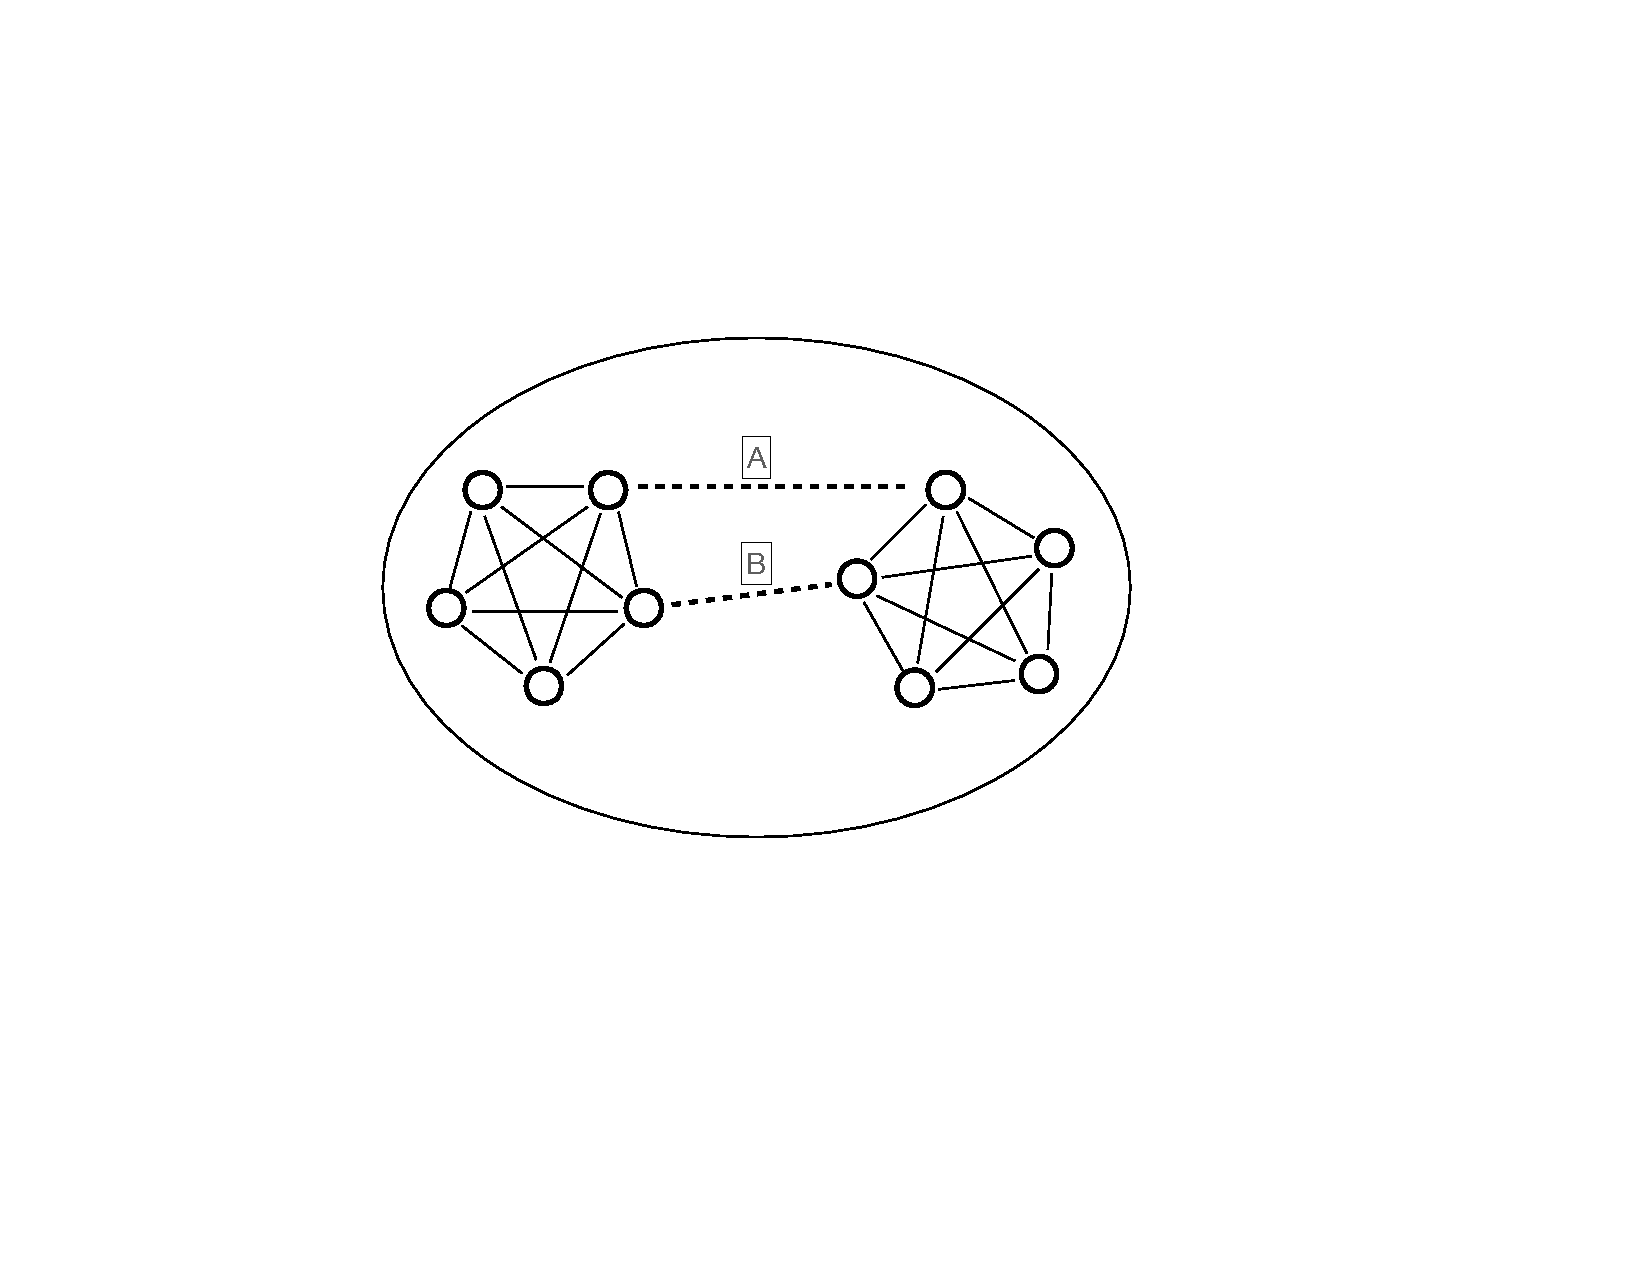
\includegraphics[width=0.5\textwidth]{figs/fig_clique.pdf}
\caption{Illustrating well-connected using Equation \ref{eqn:our-bound}. The network has two 5-cliques connected by two possible edges (dashed lines), labelled $A$ and $B$.
Each of the 5-cliques is a valid community according to Equation \ref{eqn:our-bound}, but we question whether the merger of the two 5-cliques is also valid.
According to Equation \ref{eqn:our-bound}, the minimum edge cut size  must be at least 2 for a cluster with 10 nodes to be considered well-connected.
Therefore, if only one of the edges $A$ and $B$ is present in the graph, the merged cluster  would not  be considered well-connected.
However, if both of these edges is in the network, merging the two clusters into one would produce a cluster that passes our minimum connectivity test.
On the other hand, for Equation \ref{eqn:cpm-bound}, whether the cluster formed by merging the two cliques is adequately well-connected depends on the resolution parameter, $\gamma$ (see text).}
\label{fig:2cliques}
\end{figure}

As an alternative to the bound given in Equation \ref{eqn:cpm-bound},  we consider the
following definition for well-connected.
Specifically, we require that the size of an edge cut  $E_0$  of cluster $C$ be above some function that depends only on $||C||$.
Under this definition, a cluster would be considered well-connected if every edge cut, independent of the sizes of the
two sets it creates when deleted, is large enough.
As a simple example, we consider the bound $|E_0|| > \log_{10}(||C||)$.  To enable a comparison to Equation \ref{eqn:cpm-bound}, we rewrite this  as
\begin{equation}
  ||E_0|| \geq  \lfloor \log_{10}(||C||) \rfloor +1
  \label{eqn:our-bound}
  \end{equation}
where $||.||$ denotes the number of elements in the given set and
$\lfloor . \rfloor$ is the floor (largest integer at most the size of the given value).

For example, when $||C|| \leq 9$, the bound in Equation \ref{eqn:our-bound} only enforces that the cluster be connected, when
$10 \leq ||C|| < 100$ it requires that  the cluster not have any cut edges (single edges that disconnect the cluster), etc.
This formulation offers a relatively weak bound for large clusters (i.e., when   $||C||$ is large), but does provide  a stronger constraint on small to moderate-sized clusters than the formulation based on Equation \ref{eqn:cpm-bound}.
% \textcolor{blue}{Should we write something like, ``Thus, the guarantees offered by Leiden are stronger for larger clusters, whereas, our formulation is more stringent for small to medium sized clusters.''?}

We demonstrate this concept in Figure \ref{fig:2cliques}, where we have two cliques, each of size 5, in a network; if both the dashed edges (A and B) are present, then
merging the two cliques into a single cluster meets the minimum edge connectivity requirement (which is that the minimum edge cut must be of size at least two); however,
if only one edge is present, we cannot merge the two cliques and still have adequate edge connectivity.
On the other hand, for the CPM-based guarantee, whether the cluster formed by merging the two cliques is adequately well-connected depends on the resolution parameter, $\gamma$.
For example, if $\gamma=0.1$, then even if both edges are present, the cluster would not be considered well-connected.
If instead $\gamma=0.01$, then even if only one edge is present, the cluster would be well-connected.


Thus, the two approaches provide guarantees about clusters being well-connected for different size clusters, with the first approach (Equation \ref{eqn:cpm-bound}) being a stronger
guarantee for large clusters and the second  (Equation \ref{eqn:our-bound}) a stronger guarantee for small to moderate-sized clusters.
Understanding the differences in these guarantees is important, and is part of this study.

To explore well connectedness in community detection, we performed a study to evaluate  clusters produced by two different clustering methods:
the Leiden algorithm  \citep{Traag_2019}, and Iterative K-core Clustering (IKC) \citep{,Wedell2022}.
We designed a pipeline to work with both Leiden and IKC that would ensure that all output clusters satisfy two constraints for being valid communities: (1) each cluster meets a minimum user-specified size requirement
and (2) each cluster is well-connected according to   Equation \ref{eqn:our-bound}.
Also, (3) we ensure that each cluster is produced  by applying the selected clustering method to specified subnetworks.


The pipeline takes a Leiden or IKC clustering as input and then minimally modifies the clustering to ensure that all returned clusters meet these three requirements.
To achieve this, it  first removes all clusters that fail to meet the minimum size specified by the user; we study this method using 11 for this minimum size since we consider any cluster of size at most 10
too small to be practically informative. Since any cluster that is a tree will fail our connectivity requirement when it has 10 or more vertices, we also remove all trees that remain. These two requirements are
collectively referred to as `filtering'.  After filtering, we move to the heart of the algorithm, the ``Connectivity Modifier".

Within the Connectivity Modifier, we repeatedly examine clusters to see if they are well-connected, according to our requirement.
To do this, we use the VieCut \citep{Henzinger2018,Henzinger2019}  software for finding minimum edge cuts in graphs.
If the cluster does not have a small edge cut, i.e., all its edge cuts are at least the minimum size), then the cluster is not modified by the Connectivity Modifier,
and is returned in the output. Else, the cluster is processed recursively: first we delete the small edge cut, then we recluster the components that are created using the method
specified for the input clustering and then we recurse on each cluster that is produced. At the end of this process, every cluster that remains is well-connected, by our definition.
Moreover, every cluster that we return has been produced by Leiden, either applied to the original network or to a subnetwork created by deleting small edge cuts.
Thus, this pipeline meets properties (1) and (3), as  described above.

Note that after running the Connectivity Modifier, we have a set of clusters that are all well-connected, but some of them may be below our minimum size (default: 11).
Hence, we then check the remaining clusters to see if they are too small (at most 10 nodes), and if so we remove them.  The result of this multi-stage process is a set of
clusters that meet all three required properties. Note also that we never modify an input cluster that is sufficiently large and meets our edge-connectivity requirement, and
that every cluster that is produced is a sub-cluster of the original clustering.

Using this pipeline, we evaluate clusterings produced by Leiden and IKC for a number of different networks, including two large citation networks: the Open Citations Network with 75 million vertices and
1.36 billion edges, \and the Curated Exosome Network \cite{Jakatdar_2022} with 14 million nodes and 92 million edges. In addition, we evaluate benchmark networks from the SNAP collection \cite{snapnets}. 
For Leiden clustering of real-world networks, except for cases with relatively large resolution parameter values (i.e., $r \geq 0.1$), the majority of clusters do not meet the relatively mild constraint we have for a cluster to be considered well-connected.
The trends we observe on real-world networks are very different to those observed on synthetic networks   generated by the LFR methodology, where Leiden clusters of
synthetic networks are more likely to meet the mild constraint for well-connectedness.
Other differences in trends observed between real and synthetic networks show that after restriction to well-connected clusters, node coverage in real-world networks shrinks substantially but the same is not true for synthetic networks.  Since an assumption of the LFR network generation process  is that every vertex  is in a community, the results of this study
underscore the difference between synthetic and real world networks and suggest that community structure is not globally found within real-world networks.
Thus, our study suggests the intriguing possibility that for some  real world networks, only a reduced subset may exhibit valid community structure,
thus calling into question the assumption that  clustering methods should place all nodes in communities.


\section{Materials and Methods}

\subsection{Notation and definitions}
We begin with basic notation and definitions.
\begin{itemize}
\item We assume that all networks have no self-loops and no parallel edges.
\item A cluster $C$ is a subset of the vertices in the network. The number of vertices in $C$ is denoted by $||C||$.
\item A tree cluster is a cluster that has no cycles.
\item A clustering is a partitioning of the input network vertices into disjoint sets.  Singleton clusters are typically
discarded.  The node coverage is the percentage of the network nodes that are found in non-singleton clusters.
The edge coverage is the percentage of the network edges that are found in non-singleton clusters. Here we note, as in this article, that 
node coverage and edge coverage are sometimes restricted to calculations based on clusters above some minimum size, such as $10$.
\end{itemize}

\subsection{Methods}
The pipeline we describe is modular, and requires the user to specify values for two algorithmic parameters:
\begin{itemize}
\item $B$, the minimum allowed size of any ``valid" vertex community (default $B=11$)
\item $f(n)$, a function that specifies a minimum size of an edge cut in a cluster with $n$ vertices  for the cluster to be ``well-connected" (default: $ \lfloor \log_{10} n \rfloor +1$)
\item The preferred clustering method, selected from Leiden optimizing CPM (with the resolution value $r$ provided), Leiden optimizing modularity, or the Iterative k-core (IKC) method.
\end{itemize}

\noindent
The input to the pipeline is a network $\mathcal{G}$ with $N$ nodes and the algorithmic parameters as specified.
The pipeline then operates in four stages:
\begin{itemize}
\item
Stage 1: A clustering is generated  from the input network $\mathcal{G}$,
\item Stage 2: The clustering is filtered  to remove clusters below size $B$  and any trees,
\item Stage 3: The \emph{Connectivity Modifier} (CM) is applied to each cluster that remains, which results in a set of output clusters that are well-connected (based on the function $f(n)$ provided by the user and the selected clustering method), and
\item Stage 4: We remove any resultant clusters below size $B$.
\end{itemize}
By design, this pipeline is guaranteed to return a clustering where each cluster is well-connected (according to the function $f(n)$)  and has size at least $B$.

\begin{figure}[H]
\centering
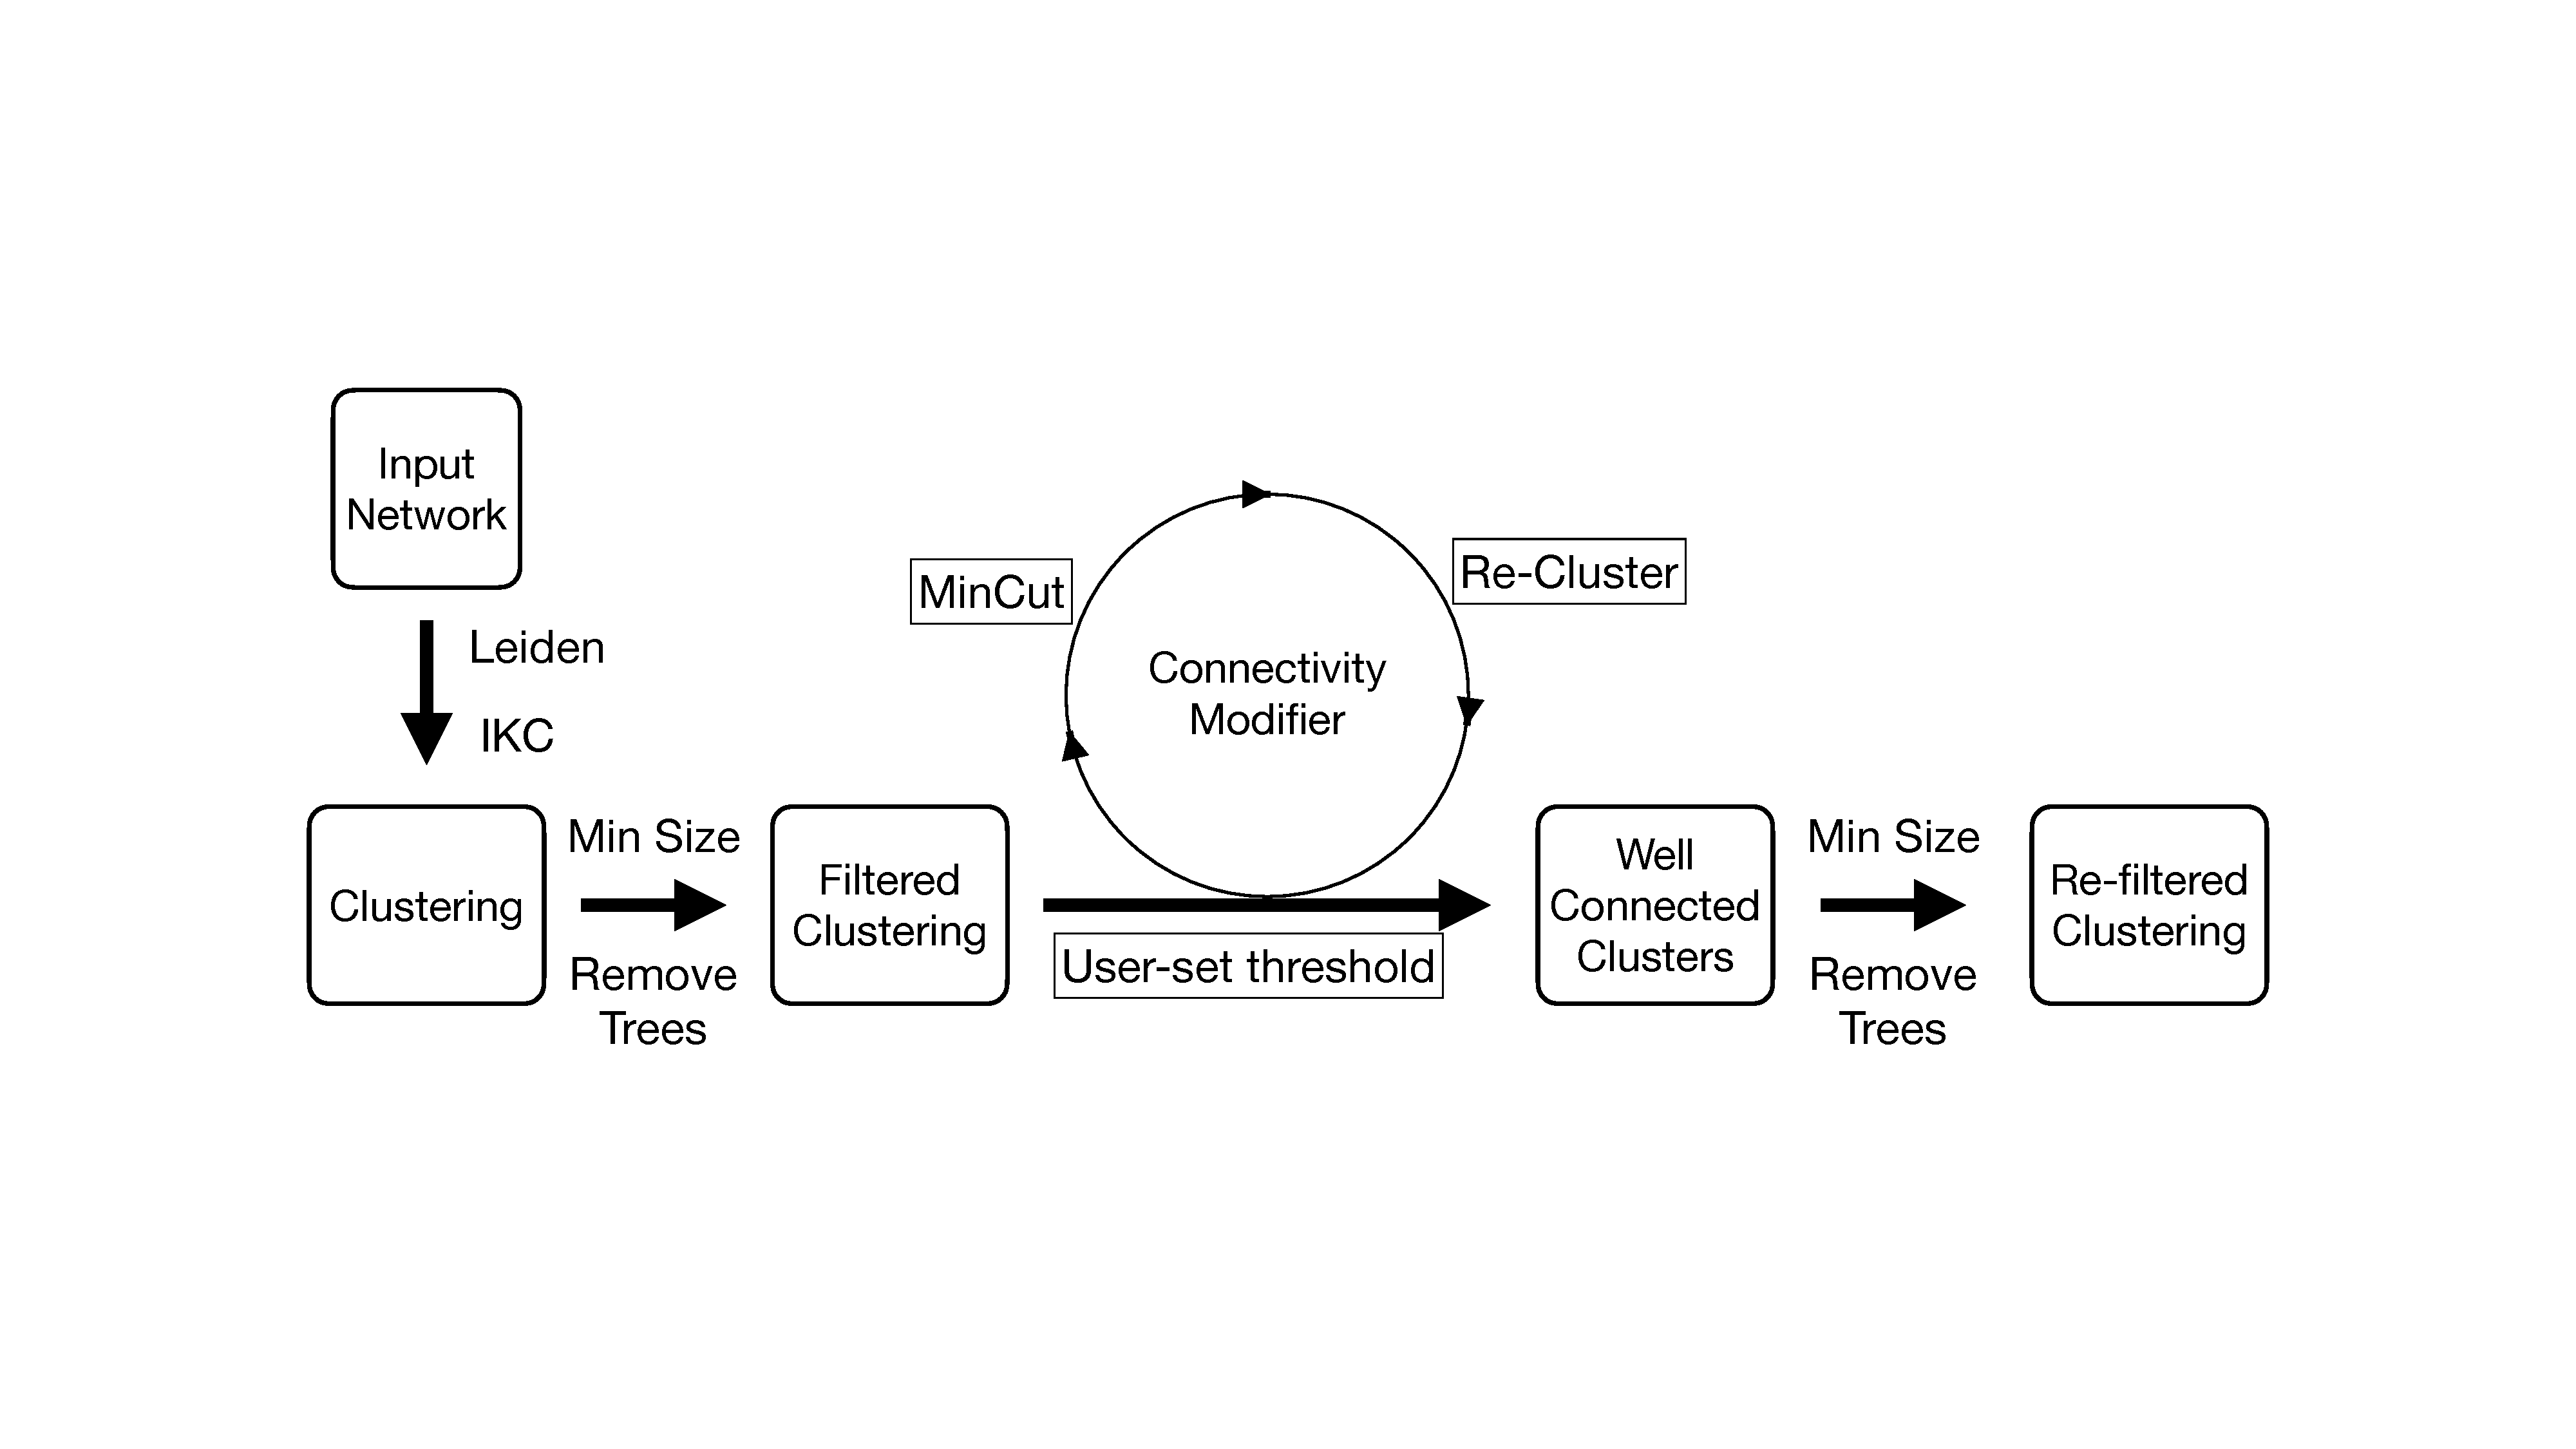
\includegraphics[width=0.8\linewidth]{figs/workflow.pdf}
\caption{Pipeline Schematic. The pipeline depends on user-specified algorithmic parameters (minimum allowed size of a cluster, required minimum number of edges in an edge cut, and clustering method), and operates in four stages:  Stage 1 computes the clustering; Stage 2 removes any clusters that are too small or that are trees;  Stage 3 runs the  Connectivity Modifier to each cluster (i.e., removing small edge cuts if they are below the required size, reclustering, and recursing),  and Stage 4 then removes the clusters that are too small. All clusters that are returned are well-connected by definition and above the minimum size, both algorithmic parameters specified by the user.}
\end{figure}




In this study, we report results using default values for the algorithmic parameters, which are: $B=11$ (so that all clusters of size at most 10 are considered too small) and requiring that the minimum edge cut for a cluster $C$ be at least  $ 1+ \lfloor \log_{10}(||C||) \rfloor$,  where $||C||$ denotes the number of vertices in $C$.
We report results using both Leiden optimizing CPM with different resolution parameter values and IKC, and we explore results on several networks.


\subsubsection{Filters} Clusters were filtered to remove trees and any cluster of size at most 10,. Many tools can achieve this; see supplementary information for details.
%using any of the following tools: (i) a custom R script, (ii) sequential or parallelized Python scripts using the Networkit library \citep{Staudt2016}, or (iii) Belinda, a Python package [cite supplementary information and insert Github reference to https://github.com/illinois-or-research-analytics/belinda] for clustering analysis.

\subsubsection{Connectivity Modifier} To recursively compute and apply minimum cuts to individual clusters, we used the Connectivity Modifier (CM) code at [insert Github reference to Connectivity Modifier], which uses Viecut \citep{Henzinger2018,Henzinger2019} as a dependency, and takes as input a clustering from either the Leiden algorithm or IKC, and returns a set of clusters that is guaranteed to be
well-connected.
We filtered the input clustering as above before passing it as input to Connectivity Modifier. [insert references https://pypi.org/project/connectivity-modifier/].

Here we describe the CM code when passed an input  Leiden clustering $\mathcal{C}$  optimizing CPM (i.e., in default mode). We note that modifying this description to describe how it works with IKC or with Leiden for modularity is straightforward.
We assume that the user has specified the value of the resolution parameter $r$ (referred to as $\gamma$ above and in some publications).
We assume that the minimum size of the edge cut is specified, but recall that our default setting specifies that any edge cut for a cluster $C$ that is at most $ \lfloor \log_{10}(||C||) \rfloor$ is ``too small".
CM used with Leiden and parameter $r$ has the following structure.


First, the set $Bin$ is initialized to the empty set  ($\emptyset$).
CM  then orders the clusters in the input clustering, and   processes each cluster in  turn.
When processing a single cluster $C$,
CM uses VieCut to find a small cut in $C$;  if the cut is too small (i.e., for our default, this means it has at most $\log_{10}(||C||)$ edges), then
we remove the edge cut from the cluster, which splits the cluster $C$ into two  subsets $A$ and $B$.
Both $A$ and $B$ are then reclustered using Leiden with the specified resolution parameter.
Every cluster that results is then recursively analyzed using the same CM pipeline, and the recursion stops when each cluster is considered well-connected.
All the clusters that are produced by this process are therefore well-connected, and are placed in the set $Bin$.

After all clusters are processed, the set $Bin$ is returned.
By design, every cluster in  $Bin$ will be well-connected (i.e., the min cut found using VieCut will be large enough, according to the user-specified criterion).
Furthermore, every cluster in the output will either be one of the input clusters or will be a subset of one of the input clusters.
Finally, every cluster in the input that meets the user-specified criteria for size and edge-connectivity will be found in $Bin$.

\begin{figure}[H]
\centering
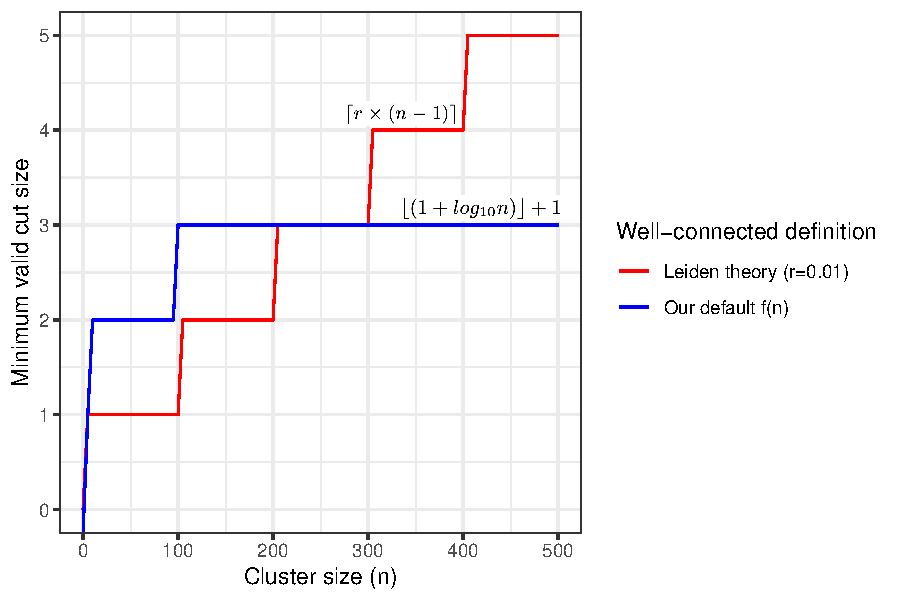
\includegraphics[width=0.7\linewidth]{figs/well_connected_definition.pdf}
\caption{Comparison of  the  lower bounds for well-connected clusters,  given in Equations \ref{eqn:cpm-bound} and \ref{eqn:our-bound}.
Equation \ref{eqn:cpm-bound} depends on the sizes of the two subsets formed by deleting the edge-cut; what we show here is based on the most imbalanced split (i.e., separating a single node from the remaining nodes in the cluster).
The figure shows two curves: the red one is for Equation \ref{eqn:cpm-bound} using $r=0.01$ and the blue one is for Equation \ref{eqn:our-bound}.
Accordingly, we see that a cluster with 200 nodes whose minimum cut is of size two, separating one node from the remaining 199 nodes, is considered well-connected
according to Equation \ref{eqn:cpm-bound}  but not according to Equation \ref{eqn:our-bound}.  However, once the cluster exceeds size 300, the lower bound for being well-connected according to
Equation \ref{eqn:cpm-bound}   is larger than the lower bound according to Equation \ref{eqn:our-bound}, making
Equation \ref{eqn:cpm-bound} a ``higher standard".
Thus, the two definitions of ``well-connected"  are meaningful in different
regions of cluster size, with Equation \ref{eqn:cpm-bound}  a higher standard on large clusters (here, above size 301) and Equation \ref{eqn:our-bound}   a higher standard on small to moderate-sized clusters (below 201).
Recall that Equation \ref{eqn:cpm-bound}  defines the lower bound for an edge cut separating one node from the remaining $n-1$ nodes
  in a cluster with $n$ vertices of $\lceil r \times (n-1) \rceil$, where $r$ is the resolution parameter (here, $r=0.01$)
and Equation \ref{eqn:our-bound} defines the lower bound on the cut size of $\lfloor(1 + log_{10}n)\rfloor +1$.}
\end{figure}

 \subsection{Data} Several networks were used for testing and analysis and were selected to provide a range of origin, size and edge density. In all cases, below the counts of nodes and edges are reported after removing duplicate records,
self-citations, and parallel edges from the source data.

\paragraph{Open Citations}
A custom-implemented ETL process was designed to process the publicly available OpenCitations dataset \citep{Peroni2020} and load it into a PostgreSQL table. Citation data was downloaded in Aug 2022. A custom ETL script, written in Bash and SQL, was used to find and pipe uncompressed CSV files, in 20 parallel jobs using the GNU Parallel command-line utility, to a custom function which loaded individual CSV files into a staging view. DOIs were also checked for case differences to remove duplicates.  The resultant network contained 75,025,194 nodes and 1,363,605,603 edges.


\paragraph{Curated Exosome Network (CEN)}
The CEN is a citation network focused on the exosome research literature consisting of 13,989,436 nodes and 92,051,051 edges. Its construction has previously been previously described in \cite{Jakatdar_2022}.

\paragraph{SNAP Networks}The following networks were downloaded from the Stanford Network Analysis Project (SNAP) website:
 (i) cit\_patents \citep{Leskovec2005}, a citation network among US patents,
%(ii) orkut \citep{Yang2013}, data from the Orkut online social network,
(ii) cit\_hepph \citep{Leskovec2005}, the Arxiv High Energy Physics paper citation network,
(iii) wiki\_talk \citep{Leskovec2010}, a network containing users and discussion from the inception of Wikipedia till January 2008,  and
(iv) wiki\_topcats \citep{Yin2017}, a web graph of Wikimedia hyperlinks.
Each network was processed to remove duplicate edges, parallel edges, and self-loops.
The numbers of nodes and edges reported in Table \ref{tab:empirical-stats-SNAP} reflect this processing.

\begin{table}[ht]
\centering
\begin{tabular}{lrrr}
  \hline
 network & edges & nodes & avg\_deg \\
  \hline
  cit\_hepph & 420,877 & 34,546 & 24.37 \\
  cit\_patents & 16,518,947 & 3,774,768 & 8.75 \\
 % orkut & 117,185,083 & 3,072,441 & 76.28 \\
  wiki\_talk & 4,659,565 & 2,394,385 & 3.89 \\
  wiki\_topcats & 25,444,207 & 1,791,489 & 28.41 \\
   \hline
\end{tabular}
% Counts manually verified on Jan 31. 2023 by gc
\caption{Empirical statistics for cleaned versions of 4 SNAP networks.}
\label{tab:empirical-stats-SNAP}
\end{table}

\paragraph{LFR (random) networks}

\textcolor{blue}{Yasamin - check the text in this paragraph}
We used the LFR software from \cite{lancichinetti2008benchmark} to create simulated networks with ground truth communities, while attempting to emulate the properties of each empirical network and its corresponding Leiden clustering. The generative model of the LFR graphs assume that the node degree and the community size distributions are power-law distributions  \citep{albert2002statistical}.
The software for generating LFR benchmark graphs\footnote{available at \href{https://www.santofortunato.net/resources}{https://www.santofortunato.net/resources}} takes the following eight parameters as input:
\begin{itemize}
    \item  \textbf{Network properties:} Number of nodes $N$, average and maximum node degrees ($k$ and $k_{max}$ respectively), and exponent for degree sequence ($\tau_1$) that is assumed to be a power-law.
    \item \textbf{Community properties:} Maximum and minimum community sizes ($c_{max}$ and $c_{min}$), and minus exponent for the community size distribution ($\tau_2$), also modeled as a power-law.
    \item Mixing parameter $\mu$, that is the ratio between the degree of a node outside its community and its total degree, averaged over all nodes in the network. Lower $\mu$ values suggest that the network is constituted from well-separated communities, as nodes are mostly connected to other nodes inside their communities, rather than outside of it.
\end{itemize}






\paragraph{Parameter Estimation.} To emulate the empirical networks using LFR graphs, we estimated all eight parameters described above for a given pair of network $\mathcal{G}$ and a clustering $\mathcal{C}$. Computing $N, k, k_{max}, c_{min}$ and $c_{max}$ is straightforward using \texttt{networkX} \citep{hagberg2008exploring}. To estimate $\mu$, we do a single iteration over all edges of the network, and for each edge, if the nodes on the two sides of it were in different communities, that edge contribute to the ratio $\mu$ of these two nodes. The total $\mu$ of the network/clustering pair is the average $\mu$ of all nodes.

To estimate $\tau_1$ and $\tau_2$, we fit a power-law distribution to the node degree sequence and the community size distribution, using the approach from \cite{clauset2009power} that is implemented in the \texttt{power-law} Python package \citep{alstott2014powerlaw}. Note that the power-law property may hold for the \textit{tail} of the degree or community size sequence and not the whole distributions. Therefore, following \cite{clauset2009power}, we estimate $x_{min}$, the minimum value for which the power-law property holds as well as the exponent $\alpha$ for the tail of the distribution. Our script for estimating these parameters is available at \href{https://github.com/illinois-or-research-analytics/cm_manuscript/tree/main/analysis/lfr-analysis}{https://github.com/illinois-or-research-analytics/cm\_manuscript/tree/main/analysis/lfr-analysis}.


\begin{table}[ht]
\caption{\textbf{Empirical statistics for LFR networks}. We provide empirical statistics for LFR networks simulated to  resemble the OpenCitations, the Curated Exosome Network (CEN), and four of the SNAP networks, using Leiden clustering with resolution parameter $r=0.01$. }
\centering
\begin{tabular}{lrrr}
  \hline
 network & nodes & edges & avg\_deg \\
  \hline
    LFR-open\_citations & 3,000,000  & 55,135,215 & 36.76 \\
    LFR-cen & 3,000,000 & 20,762,221 & 13.84 \\
    LFR-cit\_hepph &  34,546 & 431,127 & 24.95 \\
    LFR-cit\_patents & 3,774,768 & 15,640,122 & 8.29 \\
    LFR-wiki\_talk & 2,394,385 & 3,297,391 & 2.75 \\
    LFR-wiki\_topcats & 1,791,489 & 24,494,292 & 27.34 \\
 \hline
\end{tabular}
\label{tab:empirical-stats-LFR}
\end{table}

\paragraph{Generating LFR networks.}
After computing these parameters based on the Leiden clusterings of the empirical networks using selected resolution parameters (see text), we simulated LFR networks using the software from \cite{lancichinetti2008benchmark}, producing empirical statistics reported in Table \ref{tab:empirical-stats-LFR} (for a resolution parameter of 0.01). For networks with more than 10 million nodes (i.e., the OpenCitations and the CEN), we limited the number of vertices to 3 million, due to scalability limitations of  the LFR benchmark graph generator \citep{slota2019scalable}, while preserving the edge density (reflected by average degree) and the mixing parameter.  The number of nodes of the LFR graphs exactly matches the number of nodes in the corresponding empirical network. In some cases, due to the inherent limitations of the LFR graph generator, we had to modify the ranges of the community sizes (i.e., increase $c_{min}$ and decrease $c_{max}$) to generate the network.

As shown from the statistics reported in Table \ref{tab:empirical-stats-LFR} and the supplement \textcolor{blue}{add table number}, the average node degree, the mixing parameter and the exponents for the degree and community size distributions are in all cases very well-preserved. Further details about the pipeline for producing LFR graphs and the statistics of the graphs are provided in Supplementary Materials Section 2.

\section{Experimental Design}
\label{sec:expt-design}
We ran a sequence of experiments, in each case clustering networks using Leiden under CPM-optimization and with various parameter values. For some experiments we also ran the IKC pipeline.  In all cases, we explore the impact of the CM pipeline.
\begin{itemize}
\item Experiment 1: We analyze the Open Citations Network using Leiden  and IKC (k=10), followed by the CM pipeline.
\item Experiment 2: We analyze the Curated Exosome Biology (CEN) network using Leiden and IKC, followed by the CM pipeline.
\item Experiment 3: We analyze LFR networks built to resemble the Open Citations Network and the CEN network (using Leiden clusterings), using Leiden, followed by the CM pipeline.
\item Experiment 4: We analyze networks from the SNAP collection and their LFR model networks, in each case using Leiden followed by the CM pipeline.
\end{itemize}

For each experiment, we report empirical statistics, such as the distribution of cluster sizes, and node  coverage.
We will say that a cluster has a {\bf small cut} if its minimum cut is found to be below  the size specified in
 Equation \ref{eqn:our-bound}, and we will report the percentage of clusters of size at least 11 that have small cuts.


\section{Results and Discussion}
\label{sec:results-discussion}

\subsection{Experiment 1: Analyses of the Open Citations Network}

\subsubsection{Leiden analyses of the Open Citations Network}
For three different resolution values ($r=0.5, 0,1,$ and $0.01$) we computed Leiden clusterings.
The CM-pipeline steps include filtering (removing trees and clusters below size 11), followed by iteratively detecting and removing small edge cuts (ti.e., edge cuts that are below the threshold
defined by Equation \ref{eqn:our-bound}) and reclustering using Leiden.
%For each of  these three three resolution values (the largest at $r=0.5$, the smallest at $r=0.0001$, and an intermediate value of $r=0.01$),


Figure \ref{fig:oc_size_count_plots_leiden} shows the distribution of cluster sizes during the pipeline for each of these resolution values:  the input Leiden clusters (left-most column), after filtering (middle column), and after the entire pipeline completed  (right-most column).
Note that clusters of size at most 10 appeared in each input clustering, and filtering removes these clusters.
The subsequent steps in CM-processing  has no impact for the largest resolution value ($r=0.5$), but does impact the two smaller values. This is most noticeable for the smaller cluster sizes, where post-CM processed distribution is smoother than the pre-CM processed distribution.




%%%%%%%%

\begin{figure}[H]
\centering
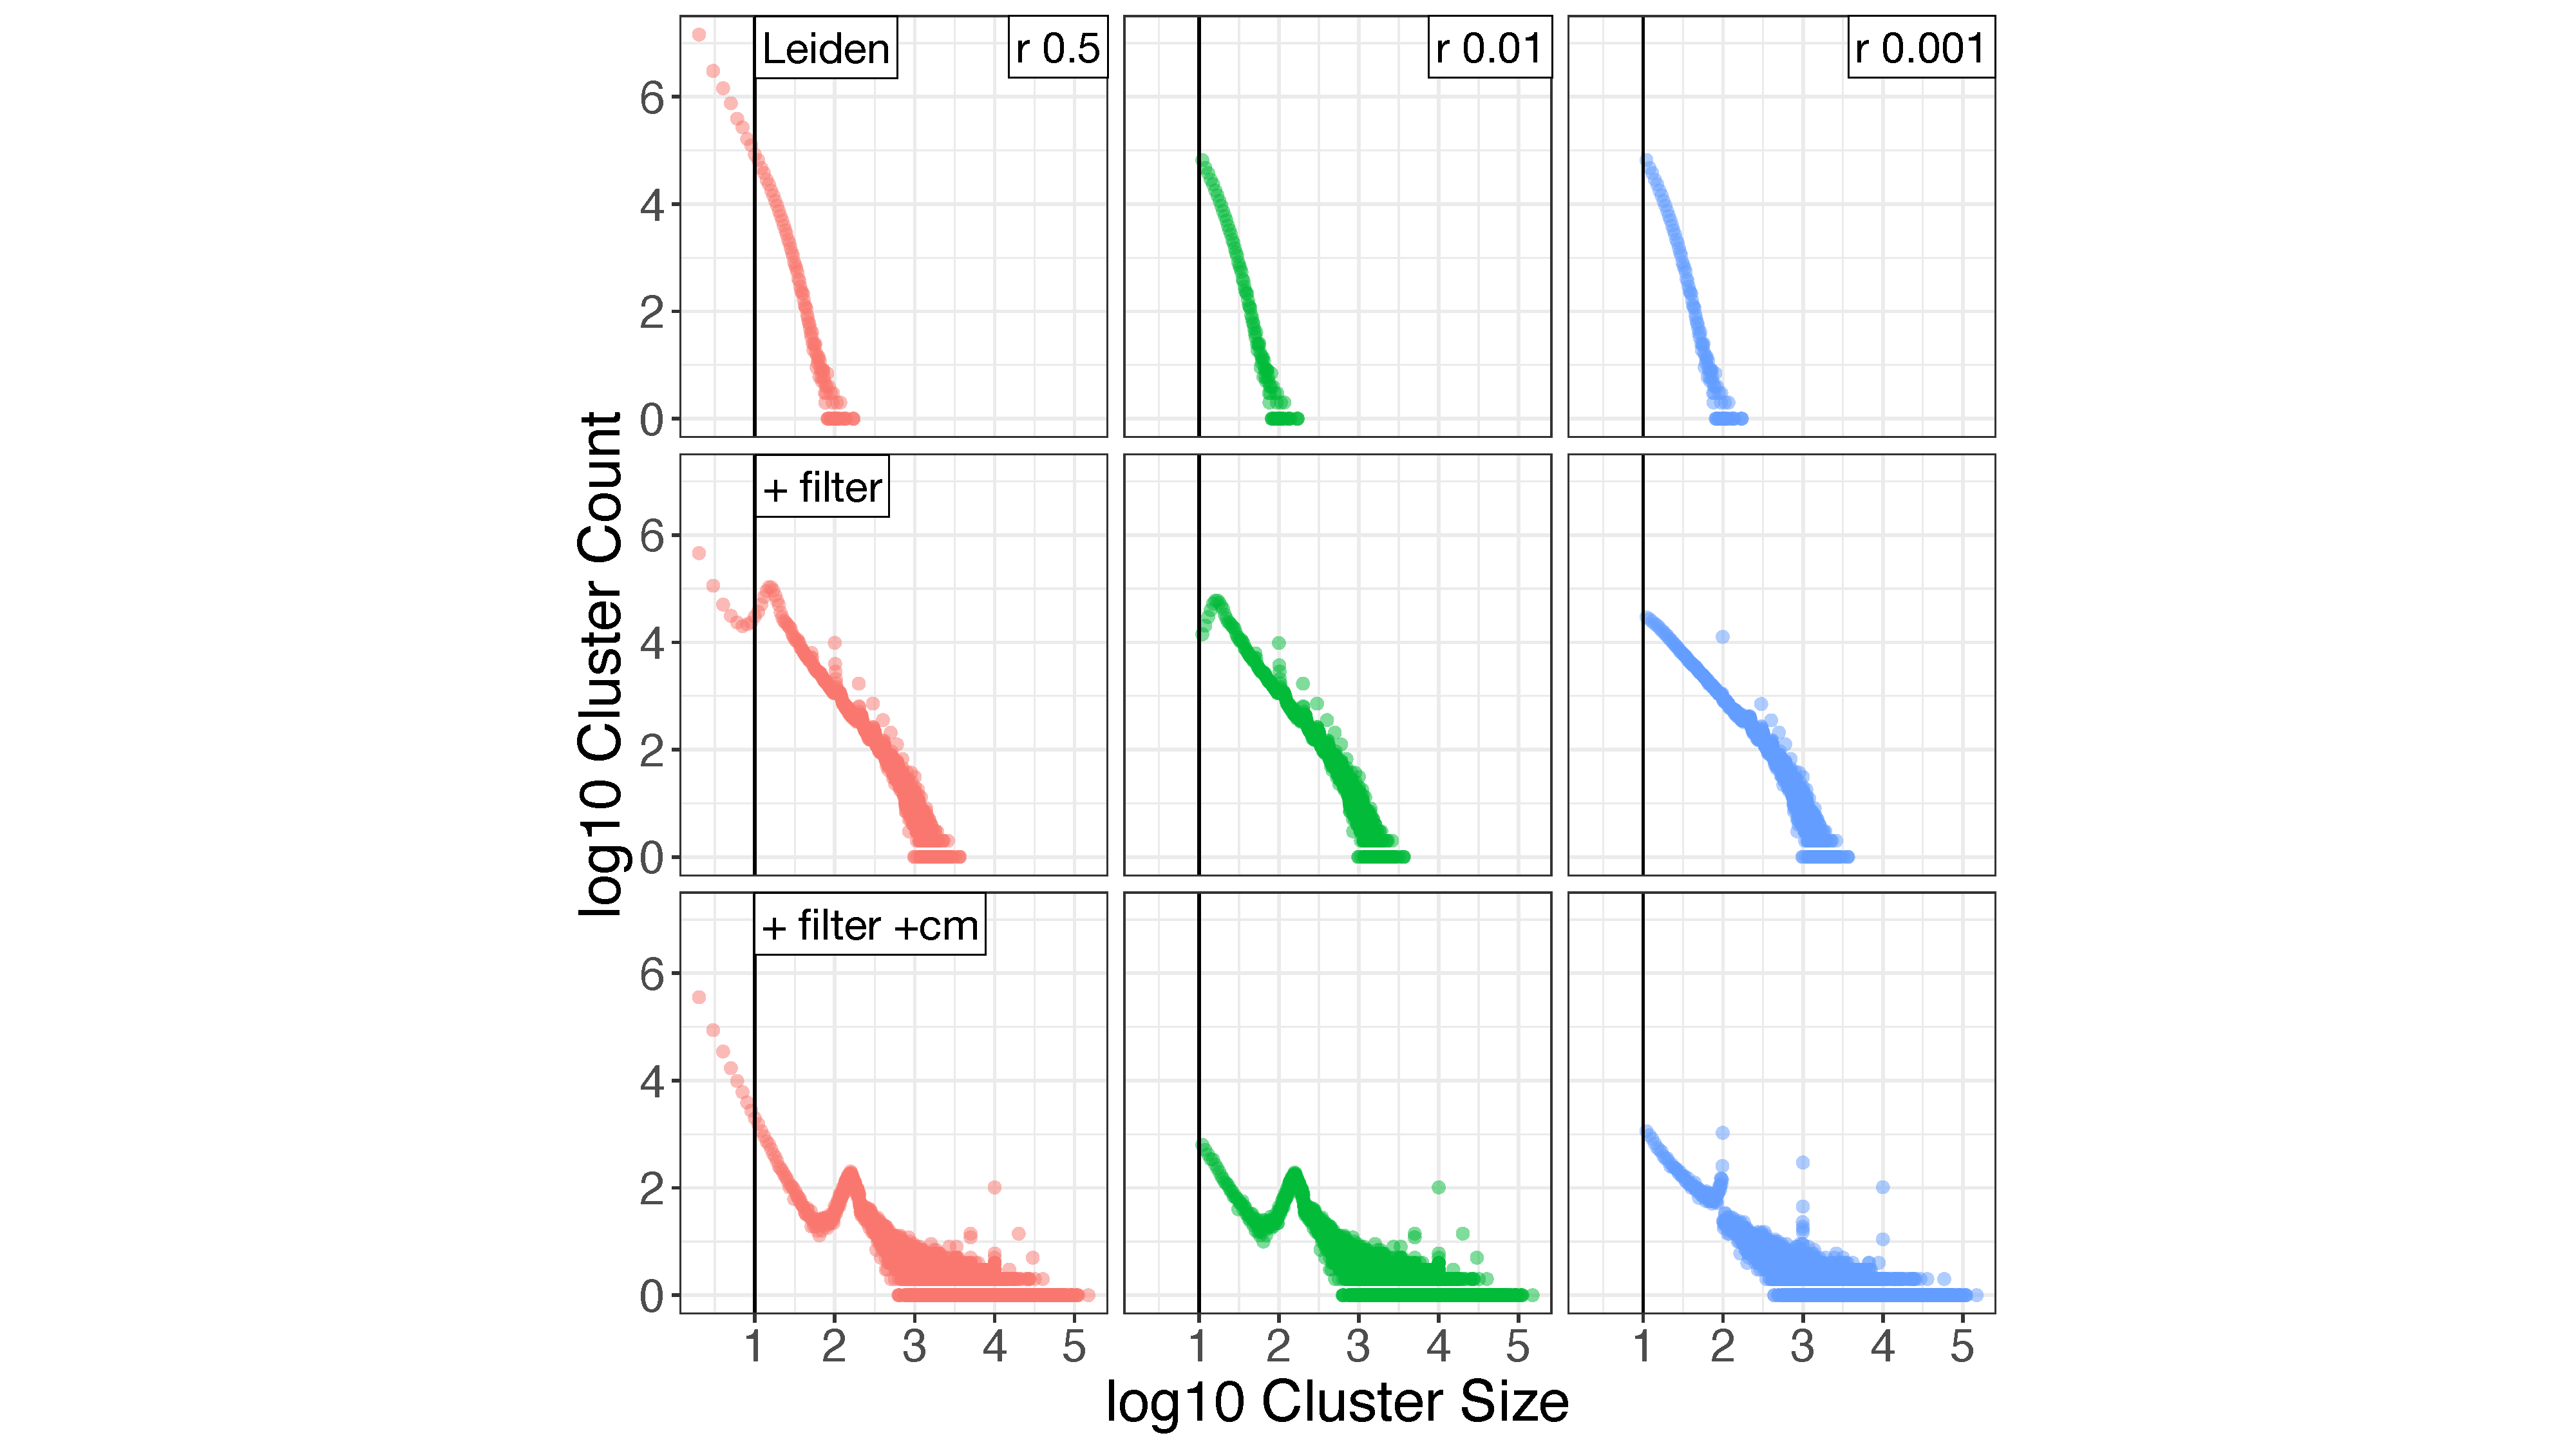
\includegraphics[width=\linewidth]{figs/fig1_kn.pdf}
\caption{\textbf{CM-processed Leiden clusterings of the Open Citations network exhibit a resolution-dependent reduction in clusters and cluster sizes.}
The Open Citations network consisting of 75,025,194 nodes and 1,363,605,603 edges was clustered using the Leiden algorithm,
with CPM as quality function; each row shows results for a particular resolution value (top: r=0.5, middle: r=0.01, bottom: r=0.0001).
The first column shows the cluster size distribution for the Leiden clustering; the middle column shows the cluster size distribution after filtering out trees and clusters of size at most 10; the right column shows the cluster size distribution after the complete CM pipeline (which includes a final filtering step to remove trees and clusters at most size 10).
The impact on Leiden clustering is largest for the two smaller resolution values.
See also   Table \ref{tab:something} and Figure \ref{fig:ocistouched}.}
\label{fig:oc_size_count_plots_leiden}
\end{figure}

\begin{figure}[H]
\centering
\begin{subfigure}[t]{0.45\textwidth}
\begin{center}
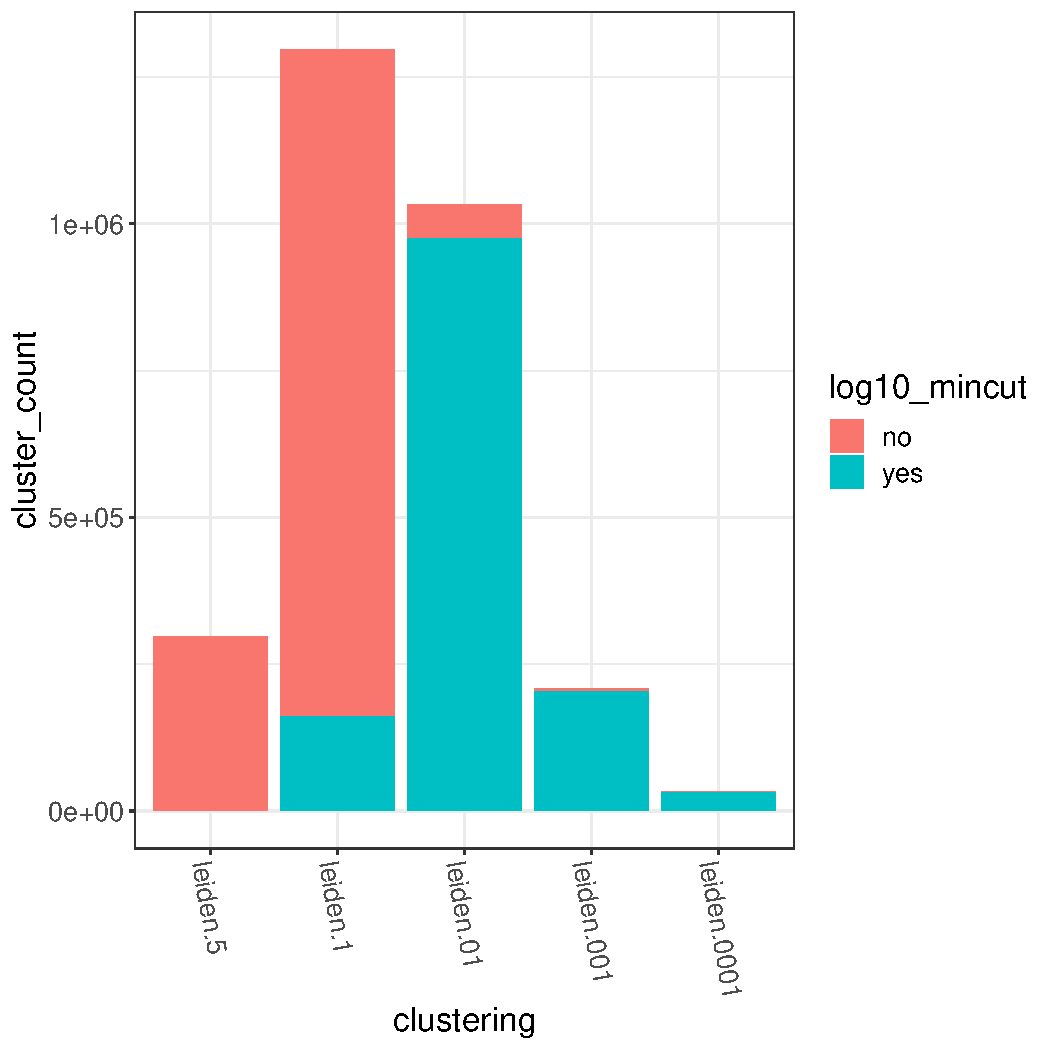
\includegraphics[width=0.9\linewidth]{figs/oc_istouched.pdf}
\caption{Number of Leiden clusters of OC}
\end{center}
\label{fig:ocistouched-part1}
\end{subfigure}
\begin{subfigure}[t]{0.45\textwidth}
\begin{center}
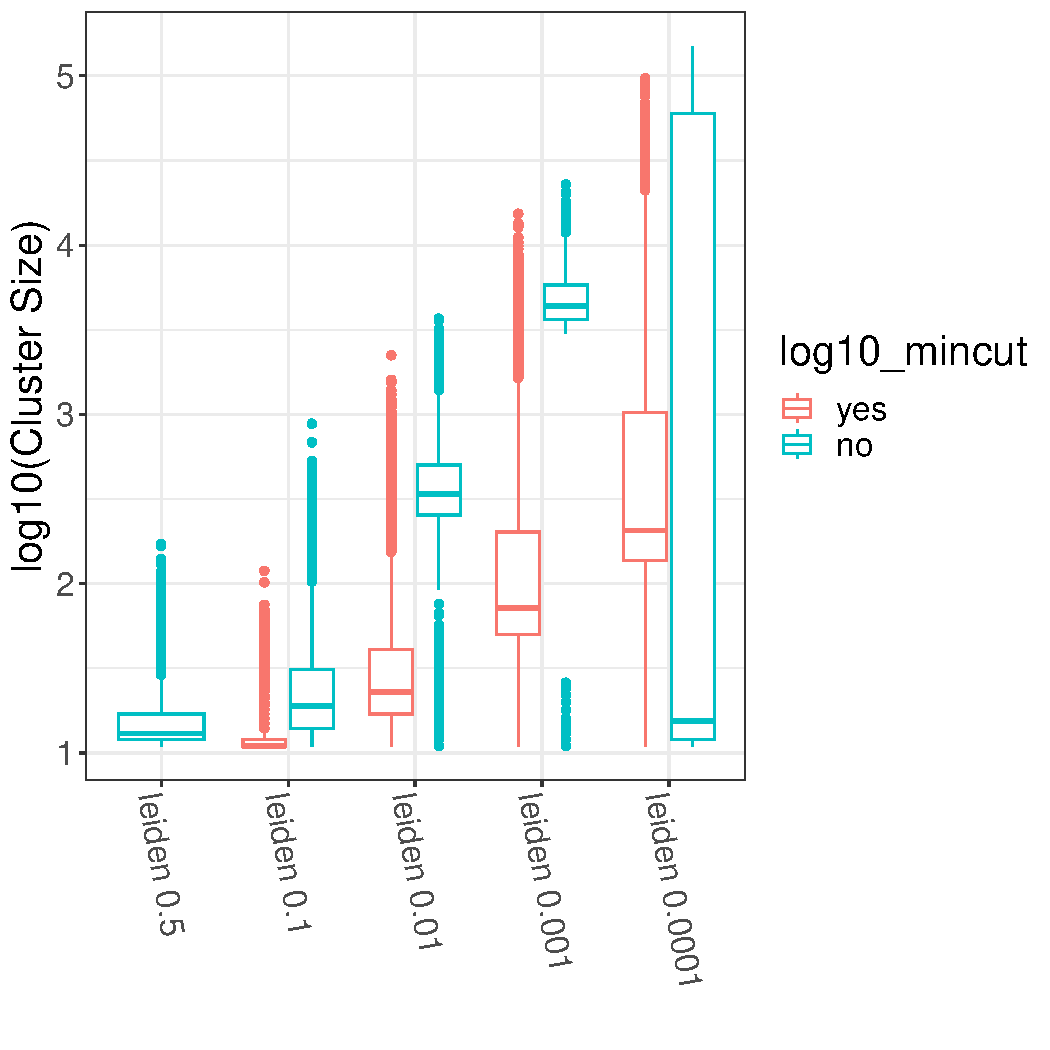
\includegraphics[width=0.9\linewidth]{figs/oc_boxplot.pdf}
\caption{Sizes of Leiden clusters of OC}
\end{center}
\label{fig:ocistouched-part2}
\end{subfigure}
\caption{\textbf {Leiden clusterings of OC} (a)
Each bar shows the total number of clusters for each of five resolution values, divided into clusters that have small edge cuts (red)  and those that do not have small edge cuts (blue), after restriction  to clusters of size at least 11. At the largest examined resolution parameter ($r=0.5$) no clusters have small cuts, but  as the resolution parameter reduces, the frequency of  small cuts increases.
For the two smallest resolution parameters show, nearly all clusters have small edge cuts.
(b)  Distributions of cluster sizes  for Leiden Clusters are shown for five resolution values, for clusters with small edge cuts (red) or without small edge cuts (blue). For all but the smallest resolution value, the clusters with small edge cuts tend to be smaller than the clusters without small edge cuts. At the smallest resolution value, this relationship switches.}
\end{figure}



% latex table generated in R 4.2.2 by xtable 1.8-4 package
% Fri Mar  3 09:18:16 2023
\begin{table}[ht]
\centering
\begin{tabular}{lccc}
  \hline
 res. & \# clusters with small cut & \# clusters without  small cut & percent clusters   \\
 & & & with small cuts \\
  \hline
  0.5 & 0 & 297755 & 0 \\
   0.1 & 163174 & 1133747 & 12.6  \\
    0.01 & 976900 & 56388 & 94.5\\
    0.001 & 205608 & 2584 & 98.6 \\
   0.0001 & 33665 &  98 & 99.7 \\
   \hline
\end{tabular}
\caption{\textbf{Count of Leiden clusters of the Open Citations Network that have small edge cuts.}}
%These values correspond to Figures \ref{fig:ocistouched-part1} and \ref{fig:ocistouched-part2}.} %min- each uster counts for oc\_istouched boxplot}
\label{tab:ocistouched-part1}
\end{table}


We examine the frequency with which clusters produced by Leiden, at different resolution values, have edge cuts that fail to meet the required minimum size, according to Equation \ref{eqn:our-bound}, and so are  impacted by CM-processing.
As seen in Figure \ref{fig:ocistouched-part1} and Table \ref{tab:ocistouched-part1}, except for the largest resolution parameter ($r=0.5$), most Leiden clusters are impacted by CM-processing, and so are not well-connected according to Equation \ref{eqn:our-bound}.
Strikingly, for the three smaller resolution parameter values between $0.01$ and $0.0001$, the fraction that have small edge cuts and so would not be considered well-connected by Equation \ref{eqn:our-bound} is very large, even close to 100\% for the two smallest resolution values.


Having noted that CM-processing impacts most clusters (except for when the resolution factor is very large), we then examined how CM-processing impacted the total number of clusters, cluster size distribution, and node coverage.
For all resolution values (Table \ref{tab:Leiden-OC-11}), there is a large reduction in the number of clusters and in the node coverage, but which stage of CM-processing impacts these statistics depends on the resolution value.
For the  two largest resolution values ($r=0.5$ and $r=0.1$), this is
due primarily (or exclusively) to the filtering stage (removal of trees and small clusters),
while  for the smaller resolution values this is due to the second stage (where poorly-connected clusters are broken and then reclustered).
We note that the maximum cluster sizes do not change as a result of this CM-processing, indicating that the very largest cluster in each analysis is well-connected (according to Equation \ref{eqn:our-bound}).
We also note that the median cluster size does change, sometimes increasing,  and sometimes decreasing.

One interesting trend revealed in this analysis is the number of tree clusters in the dataset.
That is, because all the clusters of size at most 10 are removed before being given to the CM pipeline, the filtering
step only removes clusters if they are trees.
Therefore, the drop in cluster count indicates the number of clusters of size at last 11 that are trees.
While there are no such clusters for resolution value $0.5$, at each other resolution value there are such clusters.
While the number of tree clusters varies, it can be large: and for $r=0.01$, 24\% of the clusters of size at least 11 are tree clusters.
%The number of tree clusters ranges from 14,188 (r-0.1), 328,111 (r=0.01), 23,860 (r=0.001), and 4949 (r=0.0001).

%For the largest resolution value ($r=0.5$), the initial clustering has nearly 21 million clusters, but after filtering (which removes clusters below size 11 and also removes tree clusters), the total number of clusters drops to 297,755. This filtering also reduces node coverage from 79.2\% to 6.0\%, showing that 73.2\% of the network nodes were contained in these discarded clusters.  After this filtering, however, there are no further changes, as every remaining cluster meets the minimal criterion for edge-cut size.
%At the next largest resolution value ($r=0.1$), the impact is nearly the same, with most clusters being removed during filtering, and then a non-trivial number of clusters being impacted by CM-processing (due to having edge cuts below the size requirement given by Equation \ref{eqn:our-bound}). The node coverage drops from 92.3\% before filtering to 41.6\% after CM-processing.
%At the three smallest resolution values, we see somewhat different trends. We still see the majority of clusters being removed during the filtering step (with a corresponding reduction in node coverage), but  the impact of CM-processing continues after filtering, and leads to a further reduction in node coverage.
Another interesting trend is the drop in node coverage.
When the node coverage was initially low (e.g., for $r=0.5$ node coverage was only 6\%, and for $r=0.01$ node coverage was only 43.76\$), there was either no drop or it was relatively small.
However, for the remaining resolution values, initial node coverage was never less than 88.9\%, but final node coverage was
 never more than 68.7\%.


% latex table generated in R 4.1.3 by xtable 1.8-4 package
% Fri Mar  3 19:00:17 2023
\begin{table}[ht]
\centering
\begin{tabular}{rlrrrrr}
  \hline
res\_value & pipeline\_stage & clus\_count & node\_cov & min & med & max \\
  \hline
0.5 & cluster & 297755 & 6.00 &    11 & 13 &   172 \\
 0.5 & filter & 297755 & 6.00&    11 & 13 &   172 \\
 0.5 & cm+filter & 297755 & 6.00 &    11 & 13 &   172 \\
 \hline
 0.1 & cluster & 1311109 & 43.76 &    11 & 17 &   882 \\
 0.1 & filter & 1296921 & 43.55 &    11 & 17 &   882 \\
 0.1 & cm+filter & 1167461 & 41.57 &    11 & 19 &   882 \\
 \hline
 0.01 & cluster & 1361399 & 88.93 &    11 & 19 &  3678 \\
 0.01 & filter & 1033288 & 82.20 &    11 & 24 &  3678 \\
 0.01 & cm+filter & 579753 & 63.98 &    11 & 30 &  3678 \\
 \hline
 0.001 & cluster & 232052 & 90.55 &    11 & 64 & 22808 \\
 0.001 & filter & 208192 & 89.32 &    11 & 73 & 22808 \\
 0.001 & cm+filter & 145954 & 68.70 &    11 & 64 & 22808 \\
 \hline
 0.0001 & cluster & 38712 & 91.89 &    11 & 177 & 149287 \\
 0.0001 & filter & 33763 & 91.71 &    11 & 206 & 149287 \\
 0.0001 & cm+filter & 27666 & 68.04 &    11 & 91 & 149287 \\
   \hline
\end{tabular}
\caption{\textbf{Leiden clustering and CM processing of the Open Citations Network}. For each of five resolution values, we show  the number of clusters (clust\_count) of size at least 11, node coverage (node\_cov, i.e., the percentage  of the nodes in the network found in clusters of size at least 11), and the minimum, median, and maximum of these clusters. The three stages shown include  \emph{cluster} (indicating the input clustering), \emph{filter} (the stage that removes  clusters of size at most 10 and tree clusters), and  \emph{cm+filter}, indicating that the entire CM pipeline has completed and has been re-filtered to remove clusters of size at most 10.}
\label{tab:Leiden-OC-11}
\end{table}


\subsubsection{IKC analyses of the Open Citations Network}

We used Iterative k-core (IKC) clustering with $k=10$ (thus, all nodes in all  IKC clusters are adjacent to at least $10$ other nodes in the cluster). 
After running IKC on the Open Citations Network, we had 2569 clusters covering 23.6\% of the network nodes, with a minimum cluster size of 11, median of 40, and maximum of about 6.65 million (Table \ref{tab:IKC-11-OC-basicstats}). 
Only 6.38\% of the input IKC clusters had small edge cuts, but generally the clusters that had small edge cuts tended to be larger
than the clusters that did not have small edge cuts (Figure \ref{fig:ocistouched-ikc}).
After running these clusters through CM-processing, the number of clusters increased to 3999, covering 19.5\% of the network nodes. The  median cluster size increased from 40 to 45, but the minimum and maximum did not change.

It is interesting to consider IKC clustering of the Open Citations  network presents in comparison to the Leiden clusterings of the Open Citations network.
With respect to node coverage and percentage of clusters with small edge cuts, IKC falls between Leiden with $r=0.5$ and Leiden with $r=0.1$.  
Just as Leiden at $r=0.5$ was completely unaffected by CM-processing and Leiden at $r=0.1$ was slightly affected, 
we see IKC (with $k=10$) only somewhat affected by CM-processing. 




\begin{table}[ht]
\centering
\begin{tabular}{lccccc}
  \hline
  IKC10 Clustering & clus count & node cov & min & med & max       \\ \hline
  pre-CM     & 2569       & 23.6     & 11  & 40  & 6,650,349 \\
  post-CM & 3999 & 19.5 & 11 & 45 & 6,650,067\\
  \hline
\end{tabular}
\caption[IKC clusters pre- and post-CM for the Open Citations Network]{\textbf{IKC clusters pre- and post-CM for the Open Citations Network} The Open Citations Network (Materials and Methods) consisting of 75,025,194 nodes and 1,363,605,603 edges was clustered with the IKC algorithm, with $k=10$. The node coverage pre-CM  is relatively modest at 23.6\%, and drops to 19.5\% after CM-processing.  The minimum and maximum cluster sizes do not change with CM-processing, but the median increases from 40 to 45.   Only 6.38\% of the input IKC clusters had small edge cuts.}
%Node coverage is the percentage of nodes in the network found in clusters of size at least 11. Minimum, median, and max cluster sizes, restricted to clusters of size at least 11, are shown in the last three columns. }
\label{tab:IKC-11-OC-basicstats}
\end{table}



\begin{figure}[h!]
\centering
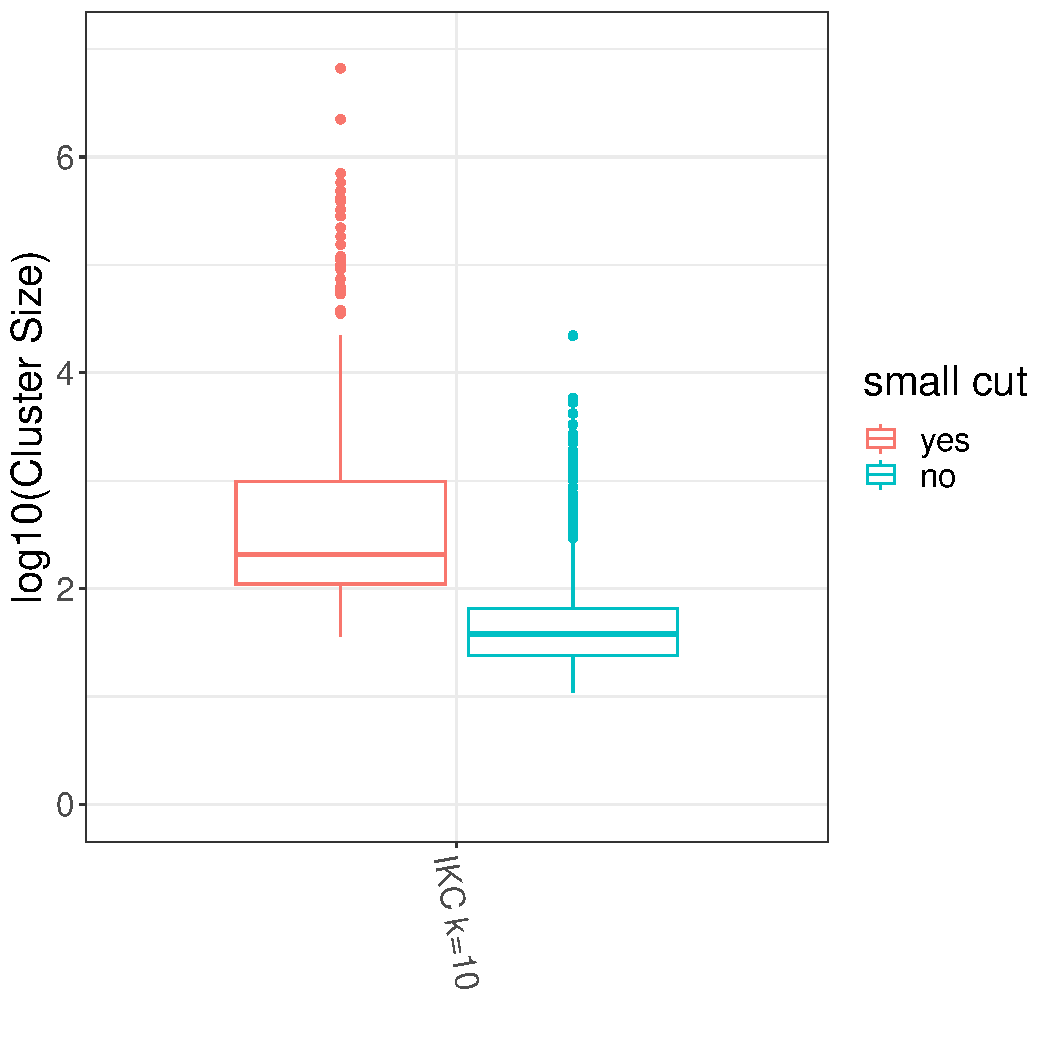
\includegraphics[width=0.37\textwidth]{figs/oc_ikc_istouched.pdf}
\caption[IKC Clusters of the Open Citations Network Impacted by CM]{\textbf{Sizes of IKC Clusters of the Open Citations Network (OC)}. For IKC clustering with $k=10$, each bar shows the distribution of cluster sizes:  red indicates those clusters that have small edge cuts and blue indicates those hat do not have small edge cuts. Only 6.38\% of the input IKC clusters had small edge cuts.
\textcolor{blue}{Minhyuk, please make the y-axis start at 0, use ylim}
.}
\label{fig:ocistouched-ikc}
\end{figure}



\clearpage
\subsection{Experiment 2: Analyses of the Curated Exosome Network (CEN)}

\subsubsection{Leiden Analyses of the CEN}

We then evaluated a citation network, the CEN (Materials and Methods) consisting of 13,989,436 nodes and 92,051,051 edges, which captures the relatively recent literature relevant to exosomes and extracellular vesicles. We clustered the CEN using Leiden optimizing CPM with  four resolution values ranging from 0.5 to 0.001 (Table \ref{tab:CEN-table1}). This range of resolution values brackets the resolution values used by us on this network in   \cite{Jakatdar_2022}.
Predictably, node coverage and cluster size increased as resolution values  decreased (Table \ref{tab:CEN-table1}).
Interestingly, the number of clusters increased and then decreased, with the smallest number of clusters for the largest
resolution value.


% latex table generated in R 4.1.3 by xtable 1.8-4 package
% Mon Jan 30 22:29:28 2023
% generated by singleton corrected script
\begin{table}[ht]
\centering
\begin{tabular}{lrrrrrr}
  \hline
 res\_value & \# clusters & min & med & max & node\_cov \\
  \hline
  0.5 &   8,503 & 11 & 14 & 68 & 0.97 \\
 0.1 &   273,420 & 11 & 11 & 319 & 23.98 \\
   0.01   & 275,641 & 11 & 28 & 3,186 & 76.52 \\
  0.001   &65,771 & 11 & 98 & 16,481 & 84.45 \\
   \hline
\end{tabular}
\caption{\textbf{Leiden clusters of size at least 11 of the Curated Exosome Network (CEN).}
For Leiden clustering under four different resolution values (left column), we show  the number of clusters of size at least 11;  the minimum, median, and
maximum cluster size when restricted to clusters of size at least $11$; and the node coverage (i.e., percentage of nodes in the CEN found in clusters of size at least $11$).
Node coverage and cluster size increase as resolution value is decreased.
\textcolor{blue}{Tandy asks: should this go into Materials and Methods? Also, this table should correspond to a table for Open Citations. It sort of does, but the
order of the columns is different. }
}
\label{tab:CEN-table1}
\end{table}


We performed the corresponding analyses on the CEN as for the Open Citations Network for these four resolution values, and report results below.
As seen in Figure \ref{fig:CEN_size_count_plots_leiden}, we see that  for each of the four resolution values, there are always some Leiden clusters  that are below
the minimum size (11), and so are removed during filtering. We also see that  the final part of the CM pipeline does not affect the distribution of cluster sizes for the
largest resolution value ($r=0.5$), has a nearly invisible impact on the second largest ($r=0.1$), but has an obvious impact for the two smaller resolution values
($r=0.01$ and $r=0.001$).
That is, before CM-processing, the distribution of cluster sizes for these two smaller resolution values shows a pattern where it starts small, increases (to a maximum somewhere
below size $100$), and then decreases; after CM-processing, the curve is smoother, and the number of clusters  decreases with the size.
These trends are similar to those seen for the Open Citations Network, but more pronounced.

We then examined the frequency of   clusters with small edge cuts for each of these parameter values (Figure \ref{fig:cenistouched-part1}).
For the largest resolution value, all clusters are well-connected, according to Equation \ref{eqn:our-bound}, but the proportion that are well-connected drops as we decrease the resolution value, so that at the two smallest resolution values nearly all clusters have small edge cuts.
This is also similar to what we observed for the Open Citations Network.

\begin{figure}[H]
\centering
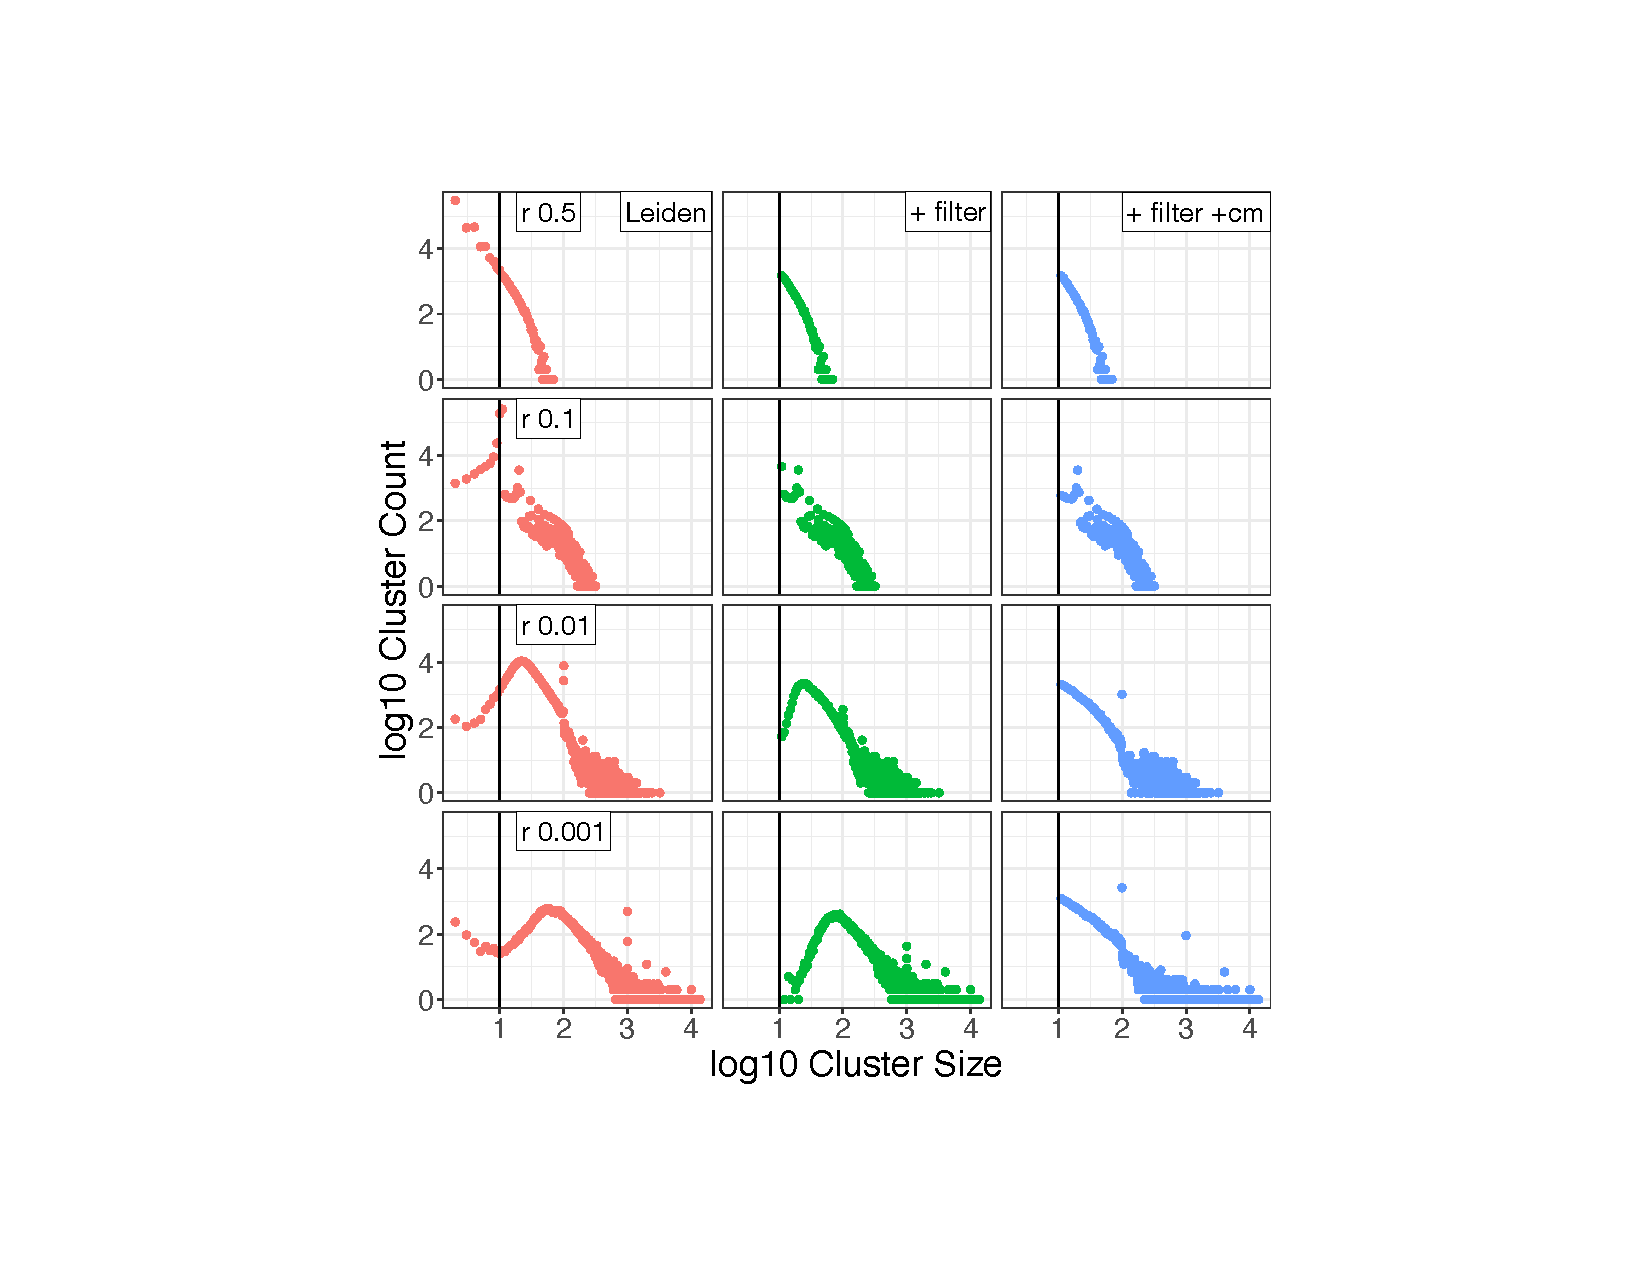
\includegraphics[width=0.8\linewidth]{figs/fig2_kn.pdf}
\caption{\textbf{CM-processed Leiden clusterings of the Curated Exosome Network (CEN) exhibit a resolution-dependent reduction in clusters and cluster sizes.}
The CEN network (with XXX nodes and YYY edges) was clustered using the Leiden algorithm, with CPM as quality function; each row shows results for a particular resolution value (top: r=0.5, middle: r=0.01, bottom: r=0.0001).
The first column shows the cluster size distribution for the Leiden clustering; the middle column shows the cluster size distribution after filtering out trees and clusters of size at most 10; the right column shows the cluster size distribution after the complete CM pipeline (which includes a final filtering step to remove trees and clusters at most size 10).
The impact on Leiden clustering is largest for the two smaller resolution values.
%The effect of filtering out tree clusters and clusters of size 10 or less and trees is shown in the middle column. The effect of subsequent treatment with CM and re-filtering is shown in the the right column.
Descriptive statistics are shown for Leiden clustering of the CEN at 5 different resolution values in Table \ref{tab:something}.}
\label{fig:CEN_size_count_plots_leiden}
\end{figure}

\begin{figure}[H]
\centering
\begin{subfigure}[t]{0.45\textwidth}
\begin{center}
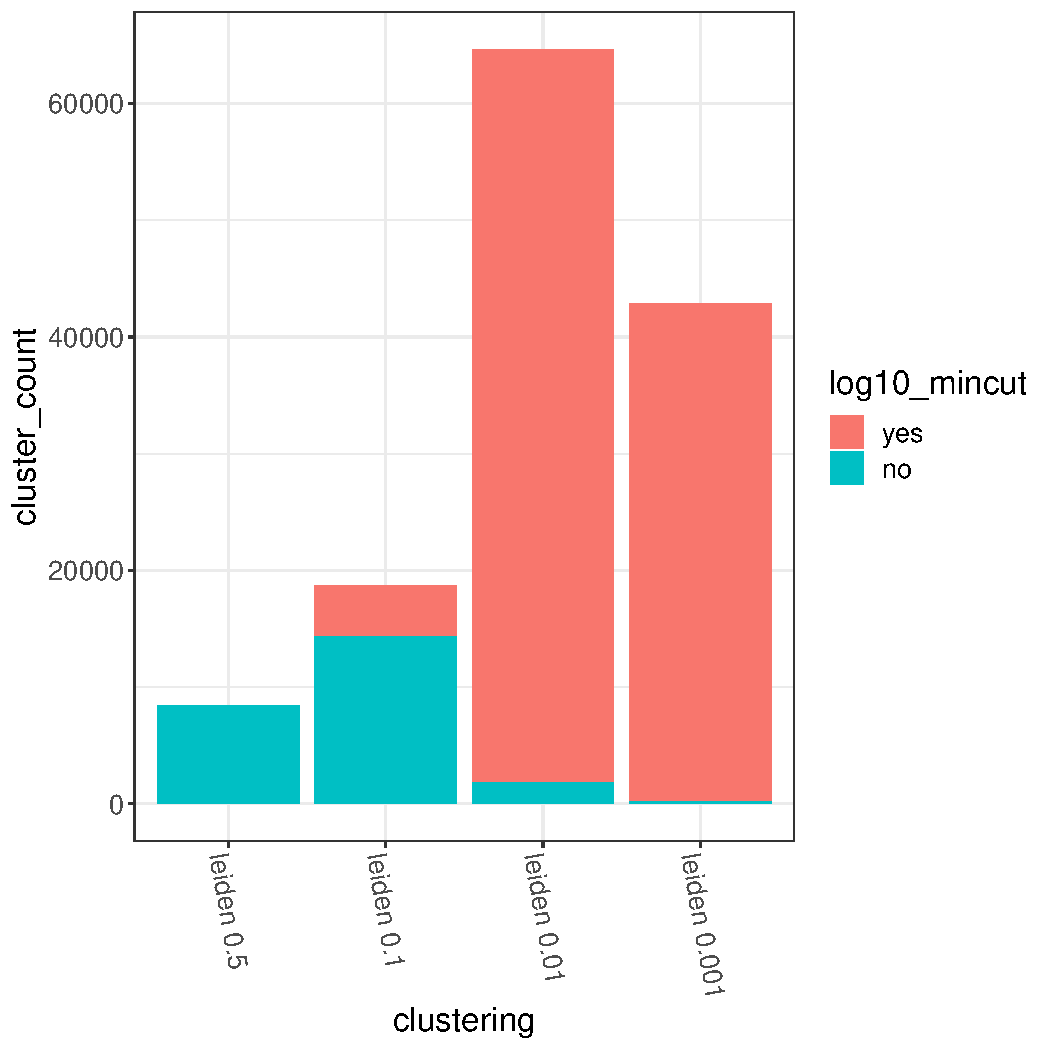
\includegraphics[width=0.9\linewidth]{figs/cen_istouched.pdf}
\caption{Number of Leiden clusters of CEN}
\end{center}
\label{fig:cenistouched-part1}
\end{subfigure}
\begin{subfigure}[t]{0.45\textwidth}
\begin{center}
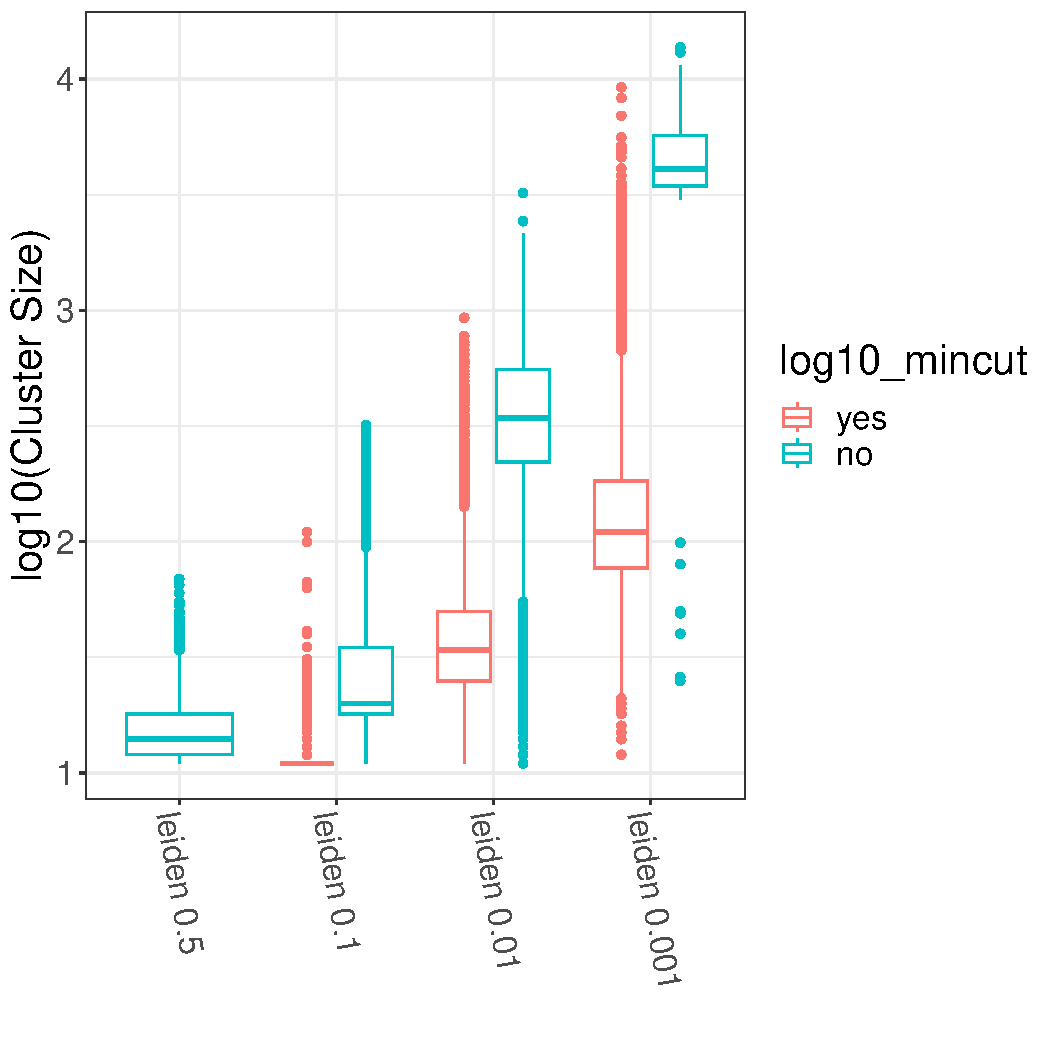
\includegraphics[width=0.9\linewidth]{figs/cen_boxplot.pdf}
\caption{Sizes of Leiden clusters of CEN}
\end{center}
\label{fig:cenistouched-part2}
\end{subfigure}
\caption{\textbf {Leiden clusterings of CEN} (a)
Each bar shows the total number of clusters for each of five resolution values, divided into clusters that have small edge cuts (red)  and those that do not have small edge cuts (blue), after restriction  to clusters of size at least 11. At the largest examined resolution parameter ($r=0.5$) no clusters have small cuts, but  as the resolution parameter reduces, the frequency of  small cuts increases.
For the two smallest resolution parameters show, nearly all clusters have small edge cuts.
(b)  Distributions of cluster sizes  for Leiden Clusters are shown for five resolution values, for clusters with small edge cuts (red) or without small edge cuts (blue). For all resolution values, the clusters with small edge cuts tend to be smaller than the clusters without small edge cuts.}
\end{figure}



% latex table generated in R 4.2.2 by xtable 1.8-4 package
% Fri Mar  3 09:27:35 2023
\begin{table}[ht]
\centering
\begin{tabular}{lrrc}
  \hline
res\_value  & yes & no & \% with small cuts\\
  \hline
  0.5 & 0  & 8406  & 0\\
  0.1 & 4357 & 14348 & 23.3\\
    0.01 & 62859 & 1806 & 97.2\\
  0.001 & 42728 & 169 & 99.6 \\
   \hline
\end{tabular}
\caption{Number of Leiden clusters of the CEN and whether they have small edge cuts}
\end{table}



% latex table generated in R 4.1.2 by xtable 1.8-4 package
% Sat Mar  4 06:26:47 2023
\begin{table}[ht]
\centering
\begin{tabular}{rlrrrrr}
  \hline
res\_value & pipeline\_stage & clus\_count & node\_cov & min & med & max \\
  \hline
0.5 & cluster &  8406 & 0.96 &    11 & 14 &    69 \\
  0.5 & filter &  8406 & 0.96 &    11 & 14 &    69 \\
  0.5 & cm+filter &  8406 & 0.96 &    11 & 14 &    69 \\
  \hline
  0.1 & cluster & 274600 & 24.05 &    11 & 11 &   319 \\
  0.1 & filter & 18705 & 3.92 &    11 & 19 &   319 \\
  0.1 & cm+filter & 14537 & 3.59 &    11 & 20 &   319 \\
  \hline
  0.01 & cluster & 275801 & 76.56 &    11 & 28 &  3217 \\
  0.01 & filter & 64665 & 24.88 &    11 & 34 &  3217 \\
  0.01 & cm+filter & 34322 & 13.22 &    11 & 24 &  3217 \\
  \hline
  0.001 & cluster & 65737 & 84.35 &    11 & 97 & 13736 \\
  0.001 & filter & 42897 & 62.13 &    12 & 110 & 13736 \\
  0.001 & cm+filter & 27363 & 23.19 &    11 & 33 & 13736 \\
   \hline
\end{tabular}
\caption{Identifying well-connected clusters from Leiden clustering of the CEN. For each of resolution values \{0.5, 0.1, 0.01, 0.001\}, clusters were limited to those of size 11 or greater, then depleted of trees, the processed by CM, and then filtered to remove any clusters of size 10 or less as well as trees. Cluster count, and min, med, and max, and node coverage refer to clusters of size at least 11.
Trends shown here reveal that node coverage is least 0.5 and at most  0.01 (Table \ref{tab:CEN-table1}. However, removal of trees and CM treatment reduces node coverage by 20.4\%, 63.3\%, and 61.3\% of the original values for resolution values of 0.01, 0.01, and 0.001 respectively.  For example, at resolution value 0.001, node coverage drops from 84.45\% to 23.15\%. At a resolution value of 0.5, no change is observed.}
\label{tab:CEN-Leiden-11-CM}
\end{table}

We then examined the impact of the CM pipeline on Leiden clusters, but restricted to those of size at least 11 (Table \ref{tab:CEN-Leiden-11-CM}).
In this case, the filtering stage only removes trees.
For the largest resolution value ($r=0.5$), there are no changes in the clustering at any step of the CM-pipeline.
However, for all the other resolution values we explore, filtering reduces the number of clusters by a substantial amount (e.g., from 273,420 clusters to 18,686 when using $r=0.1$), showing that the number of clusters that are trees is very large.
The maximum cluster size does not change for any of these resolution values, indicating that these specific clusters are well-connected according to
Equation \ref{eqn:our-bound}, but the median cluster sizes do change (sometimes increasing, sometimes decreasing).

Node coverage also drops substantially after filtering and then again after the pipeline completes.
For example,
node coverage begins at 84\% for $r=0.001$, drops to 62\% as a result of filtering, and then drops to 23.15\% by the end of the
pipeline.
Furthermore,
across all resolution values we explored, the node coverage after CM-processing was never more than 23.15\%.

\paragraph{Comparing Experiments 1 and 2}
Overall, the  trends seen for Leiden clusterings on the CEN are  very similar to what we observed for the Open Citations network.
Specifically, for both networks, we observe the following consistent trends that depend on whether one is using small resolution values ($r \leq 0.01$) or large values
($r \geq 0.1$):
(1) when using small resolution values,  nearly all Leiden clusters have small edge cuts and there is a large drop in node coverage produced by the CM-pipeline, (2) when using
large resolution values, there is less impact (or perhaps no impact) produced by the CM-pipeline, but the node coverage is small (and the clusters themselves tend to be small).
The main difference between results on the CEN and Open Citations is that the reduction in node coverage produced by CM-processing is
much larger  for the CEN than for Open Citations.
% latex table generated in R 4.2.2 by xtable 1.8-4 package
% Sun Jan 15 17:37:03 2023

% latex table generated in R 4.2.2 by xtable 1.8-4 package
% Fri Jan 13 18:03:02 2023


\subsubsection{IKC analyses of the CEN}
 
 

We used Iterative k-core (IKC) clustering with $k=10$ (thus, all nodes in all  IKC clusters are adjacent to at least $10$ other nodes in the cluster). 
After running IKC on the CEN we had 128 clusters covering 3.8\% of the network nodes, with a minimum cluster size of 14, median of 79, and maximum of about 214,877 (Table \ref{tab:IKC-11-CEN-basicstats}). 
\textcolor{blue}{Only X\% of the input IKC clusters had small edge cuts. 
 A comparison of cluster sizes with or without small edge cuts is shown in BLAH- BLAH BLAH.}
 After running these clusters through CM-processing, the number of clusters increased to 187 but node coverage is unchanged at 3.8\%.   The  minimum cluster size does not change, the median drops from 79 to 64, and the maximum cluster size drops from 214,877 to 214,850. 
 %median cluster size increased from 40 to 45, but the minimum and maximum did not change.

It is interesting to consider IKC and Leiden clustering of the CEN. 
\textcolor{blue}{Check this next text for correctness.}
With respect to node coverage and percentage of clusters with small edge cuts, IKC falls between Leiden with $r=0.5$ and Leiden with $r=0.1$.  
Just as Leiden at $r=0.5$ was completely unaffected by CM-processing and Leiden at $r=0.1$ was slightly affected, 
we see IKC (with $k=10$) only somewhat affected by CM-processing. 



\begin{table}[ht]
\centering
\begin{tabular}{rrrrrr}
  \hline
Clustering & clus count & node cov & min & med & max       \\ \hline
pre-CM       & 128         & 3.8       & 14  & 79  & 214,877 \\
post-CM & 187 & 3.8 & 14 & 64 & 214,850\\
  \hline
\end{tabular}
\caption[IKC clusters pre- and post-CM processing for the CEN]{\textbf{IKC clusters  for the CEN}
The Curated Exososome Network was clustered with the IKC algorithm using  $k=10$.
%Results 
%Node coverage is the percentage of nodes in the network found in clusters of size at least 11. Minimum, median, and max cluster sizes, restricted to clusters of size at least 11, are shown in the last three columns.}
}
\label{tab:IKC-11-CEN-basicstats}
\end{table}



\subsection{Experiment 3: Analyses of LFR networks based on the Open Citations and CEN networks}



In this experiment, we analyze synthetic networks simulated to reproduce the empirical statistics of the Open Citations and CEN networks, using the
LFR software.
However, due to limitations in network sizes that can be feasibly achieved using LFR, these synthetic networks are smaller than the corresponding
empirical networks, but have very close mixing parameters and average degrees.
\textcolor{blue}{Say where the tables are with this info.}


We begin with a comparison  between LFR and empirical networks for Open Citations and CEN networks, with respect to percentage of  Leiden clusters (using $r=0.01$) that have small edge cuts and in
the node coverage (both before and after CM-processing).   As seen in
Table \ref{tab:LFR-vs-empirical-OC-CEN}, nearly all of the Leiden clusters of these empirical networks have small edge cuts (94.5\% for the Open Citations and 97.2\% for the CEN).
\textcolor{blue}{In contrast, these percentages drop to XXX and YYY, respectively, on the LFR versions of the Open Citations and CEN networks.}
Node coverage is also different between the empirical networks and their LFR variants: before CM-processing, the node coverage begins at 88.9\% for the Open Citations and 76.6\% for the CEN, and then drops to 63.98\% and 13.22\%, respectively, after CM-processing. 
\textcolor{blue}{However, on the LFR networks, node coverage begins close to 100\% and drops only slightly.}
Thus, there are very large differences between these LFR and empirical networks.

\begin{table}[ht]
\centering
\begin{tabular}{lccc}
  \hline
 network & \% with small cuts & node cov.~pre-CM (\%) & node cov.~post-CM (\%) \\
   \hline
   CEN  &97.2 &76.56 &13.22 \\
   CEN (LFR) &  & 98.75 & 88.95\\
   \hline
   Open Citations  &94.5&88.93&63.98 \\
   Open Citations (LFR) &&&\\
   \hline
\end{tabular}
% Counts manually verified on Jan 31. 2023 by gc
\caption{\textbf{Comparing Leiden clusters before and after CM-processing  on   OC and CEN networks.} W compare statistics for Leiden clustering (using $r=0.01$) before and after CM-processing on the empirical networks and their LFR model
networks for the Open Citations (OC)  and Curated Exosome Network (CEN). We show the percentage of clusters with small edge cuts, the node coverage before CM processing (but after removing clusters of size at most 10), and the node coverage
after CM processing.  By design, the reduction in node coverage due to CM processing  is therefore due only to clusters having small edge cuts.}
\label{tab:LFR-vs-empirical-OC-CEN}
\end{table}

In the bottom row of Figures \ref{fig:oc-cm-lfr-001} and  \ref{fig:cen-cm-lfr-01} we see the result of using the CM-pipeline on the LFR network based on the Open Citations  and CEN networks, respectively, each using Leiden clustering with
resolution value $r=0.001$.
For the LFR version of the Open Citations network, the input Leiden clustering has one cluster of size 10, but this is deleted during the filtering stage, and then no subsequent change occurs.
For the LFR version of the CEN network, the input Leiden clustering has four clusters of size less than 11 that are  deleted during the filtering stage, and there is a small change to the distribution of cluster sizes at the low end (e.g., between 11 and perhaps 50) as a result of the final stage of CM-processing.
Thus, for both synthetic networks, other than the Filtering step (which does find and remove a small number of trees and clusters below size 11), there is only a little
impact produced using CM-processing.

We now compare these to the corresponding Leiden clusterings for the empirical networks, examining the top rows of these two figures.
In each case we see much bigger impacts, both from the filtering step (indicating that there are many more  trees and small clusters in the Leiden clusterings of the empirical
networks) and in the subsequent steps (finding and removing small edge-cuts and then reclustering).
Moreover, the distributions of cluster sizes for the empirical networks are different at each stage of the CM pipeline than the distributions of cluster sizes for the LFR networks.

Thus, this experiment shows distinct differences between these synthetic LFR networks and the empirical networks on which they were based.
These differences occur both in the distributions of cluster sizes of the Leiden clusters before CM as well as the impact of CM-processing, where CM-processing has a larger impact on the empirical networks than on the synthetic networks.






\begin{figure}[h!]
\centering
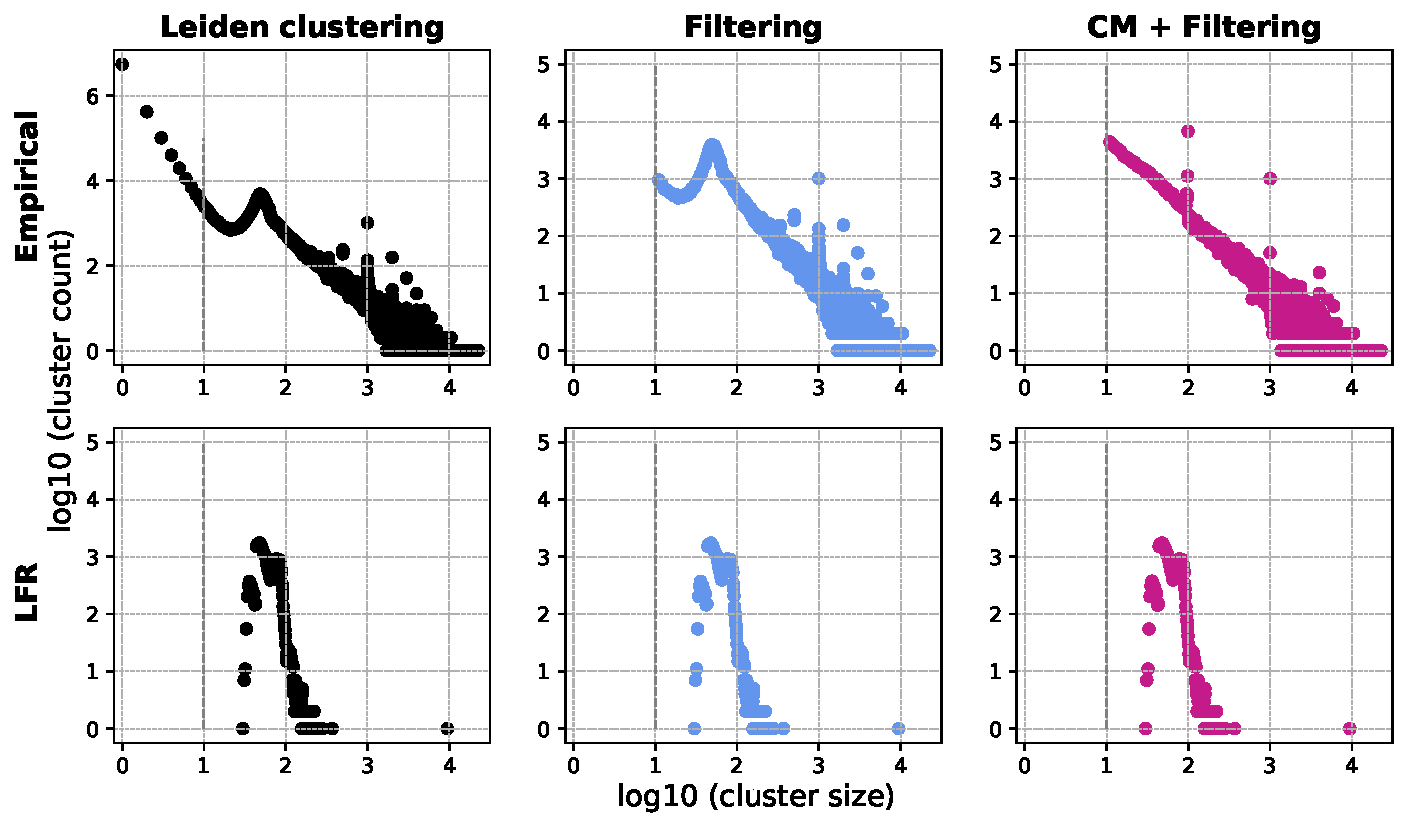
\includegraphics[width=0.62\textwidth]{figs/oc_cm_steps_lfr001.pdf}
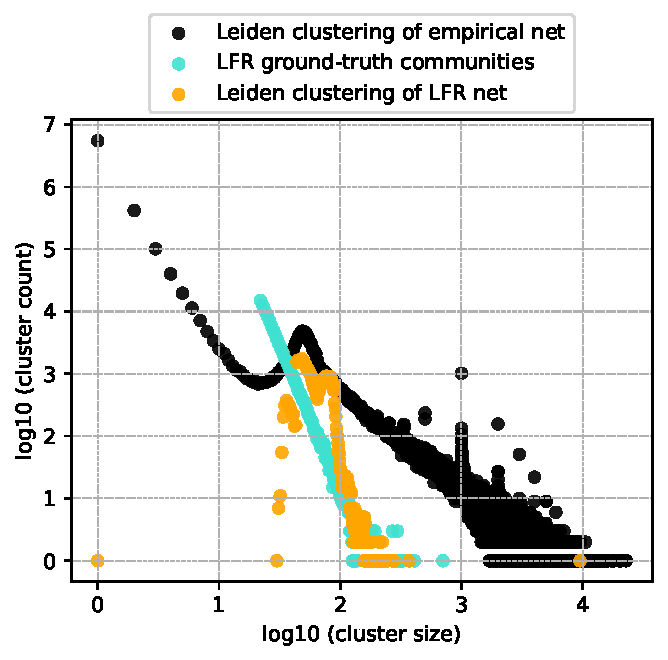
\includegraphics[width=0.37\textwidth]{figs/oc_001_cm_size.pdf}
\caption[CM pipeline on the empirical Open Citations network and its model LFR graph for r=0.001]{\textbf{CM pipeline on the empirical Open Citations network and its model LFR graph for r=0.001.} The number of nodes in the empirical network is 75,025,194 and in the LFR network is 3,000,000, but they have very close average degrees (36.34 and 36.63 respectively) and mixing parameters (0.500 and 0.501 respectively). The left panel shows the community size distribution in each step of running CM and the right panel shows a comparison between the community size distribution of the original Leiden clustering, the LFR ground-truth communities and the Leiden clustering of the LFR network.}
\label{fig:oc-cm-lfr-001}
\end{figure}




\begin{figure}[h!]
\centering
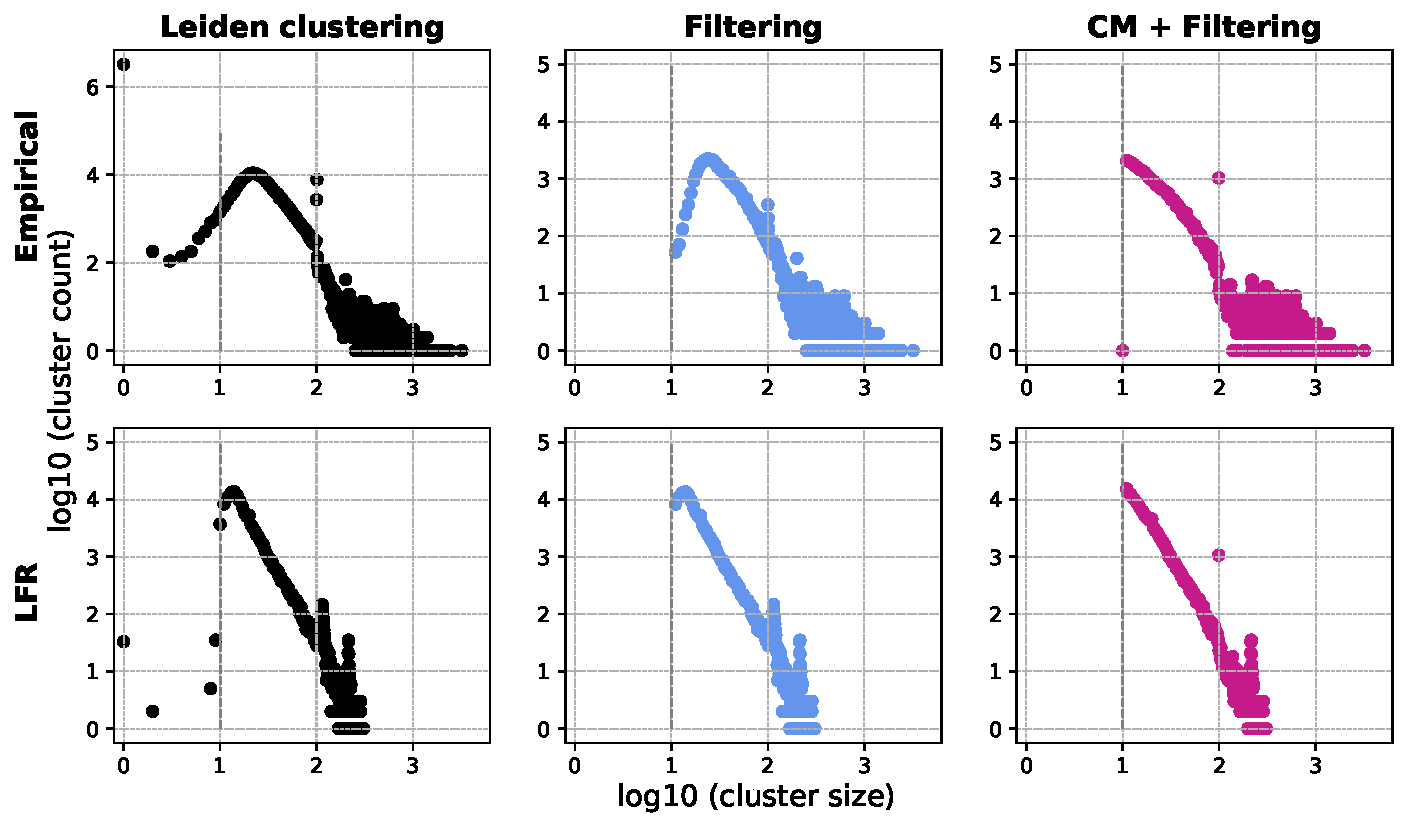
\includegraphics[width=0.62\textwidth]{figs/cen_cm_steps_lfr01.pdf}
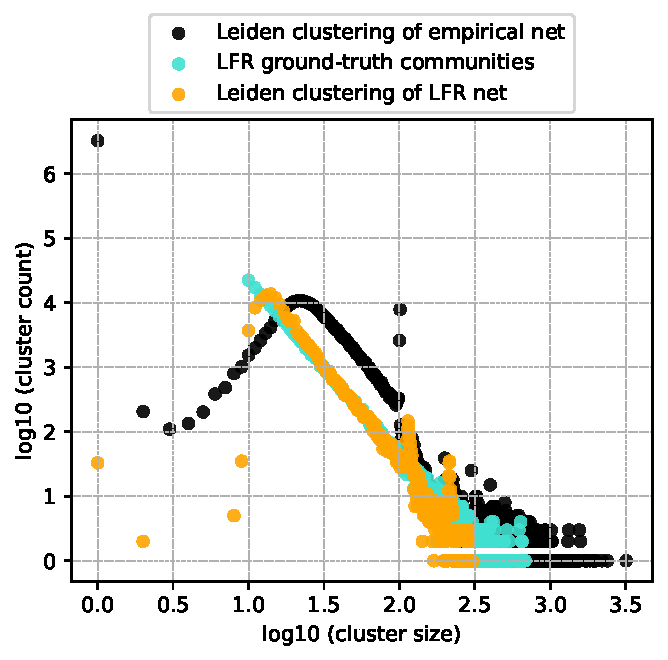
\includegraphics[width=0.37\textwidth]{figs/cen_01_cm_size.pdf}
\caption[CM pipeline on the empirical CEN network and its model LFR graph for r=0.01]{\textbf{CM pipeline on the empirical CEN network and its model LFR graph for r=0.01.} The number of nodes in the empirical CEN network is 13,989,436 nodes and in the LFR graph is 3,000,000, but they have very close average degrees (3.16 and 3.84 respectively) and mixing parameters (0.645 and 0.646 respectively). The left panel shows the community size distribution in each step of running CM and the right panel shows a comparison between the community size distribution of the original Leiden clustering, the LFR ground-truth communities and the Leiden clustering of the LFR network.}
\label{fig:cen-cm-lfr-01}
\end{figure}

\subsection{Experiment 4: Analyses of SNAP networks and their LFR model networks}

We now examine the impact of CM-processing on Leiden clusterings of four  networks from the SNAP collection, as well as of
Leiden clusterings of synthetic networks built to resemble these SNAP networks.
Because these four networks are not too large, the empirical networks have the same number of nodes as the corresponding empirical networks.


\textcolor{blue}{In Table \ref{tab:LFR-vs-empirical-SNAP}, we show some summary statistics about the  Leiden clusterings before and after CM-processing for the SNAP networks and their LFR model networks.  For each clustering of each network, we  show (a) percentage of input clusters that have small cuts, (b) node coverage prior to CM-processing, and (c) node coverage after CM-processing.  Note that
XXX and YYY.}


\begin{table}[ht]
\centering
\begin{tabular}{lccc}
  \hline
 network & \% with small cuts & node cov.~pre-CM (\%) & node cov.~post-CM (\%) \\
  \hline
  cit\_hepph  &  & 91.54 & 83.10 \\
  cit\_hepph (LFR) &  & 100.00 & 100.00 \\
  \hline
  cit\_patents & & 95.50 & 54.65\\
    cit\_patents  (LFR) & & 97.88 & 95.39\\
  \hline
 % orkut & 117,185,083 & 3,072,441 & 76.28 \\
  wiki\_talk & & & \\
    wiki\_talk (LFR) & & & \\
  \hline
  wiki\_topcats & & 91.44 & 55.49 \\
   wiki\_topcats  (LFR)& & 99.75 & 88.58 \\
   \hline
\end{tabular}
% Counts manually verified on Jan 31. 2023 by gc
\caption{\textbf{Comparing Leiden clusters before and after CM-processing  on SNAP networks.} For each of the four SNAP networks
examined in this study, we compare statistics for Leiden clustering (using $r=0.01$) before and after CM-processing on the empirical networks and their LFR model
networks. We show the percentage of clusters with small edge cuts, the node coverage before CM processing (but after removing clusters of size at most 10), and the node coverage
after CM processing.  By design, the reduction in node coverage due to CM processing  is therefore due only to clusters having small edge cuts.}
\label{tab:LFR-vs-empirical-SNAP}
\end{table}



In Figure \ref{fig:patents-cm-lfr-01}, we show results on the Citation Patents Network  (with 3,774,768 nodes), with results for the
empirical  network in the top row and results on the LFR network in the bottom row.
Corresponding results are shown for the Wiki Topcats network in Figure \ref{fig:wikitopcats-cm-lfr-01}, for the High Energy Physics Citation network
in Figure \ref{fig:hepph-cm-lfr-01}, and for the Wiki Talk network in Figure\ ref{something}.



Beginning with the results for the empirical Citation Patents Network (Figure \ref{fig:patents-cm-lfr-01}), we that the shape of the curve begins with a large number of very small clusters, then decreases and increases to a maximum
at about \textcolor{blue}{25?}, after which it decreases.
Filtering removes small clusters, producing a distribution where there is an initial increase in number of clusters
followed by a decrease.  The final  steps of CM-processing then smooth out the curve so that the number of clusters decreases as the size increases.
Thus, CM-processing has a similar impact on this network as observed on the Open Citations and CEN network.

The same process on the LFR network (bottom row Figure \ref{fig:patents-cm-lfr-01}) shows  somewhat different trends.
First, the shape of the curve is different: it begins now, increases, and then decreases.
We note that filtering removes a small number of clusters below size 11, and that
after filtering, there is a very brief interval in which the number of clusters increases.
The final stage of CM-processing smooths out the distribution.
Thus, there is a difference between the empirical and synthetic networks, both in terms of the initial Leiden clustering and the impact of each of
the stages of CM-processing.

We now briefly describe the trends on the other SNAP networks and their LFR versions.
The trends seen for the Wiki-Topcats networks  (Figure \ref{fig:wikitopcats-cm-lfr-01}) are very similar to those seen for the Citation Patents
Network, but here we also see that the Leiden clustering on the empirical Wiki-Topcats network produces larger clusters than the Leiden clustering on the LFR version.
On the High Energy Physics Citation Network (Figure \ref{fig:hepph-cm-lfr-01}), there are somewhat bigger differences between the LFR and empirical networks, with the Leiden clustering of the empirical network producing many smaller clusters than the Leiden clustering on the LFR network (which had no clusters below size 11).



\begin{figure}[h!]
\centering
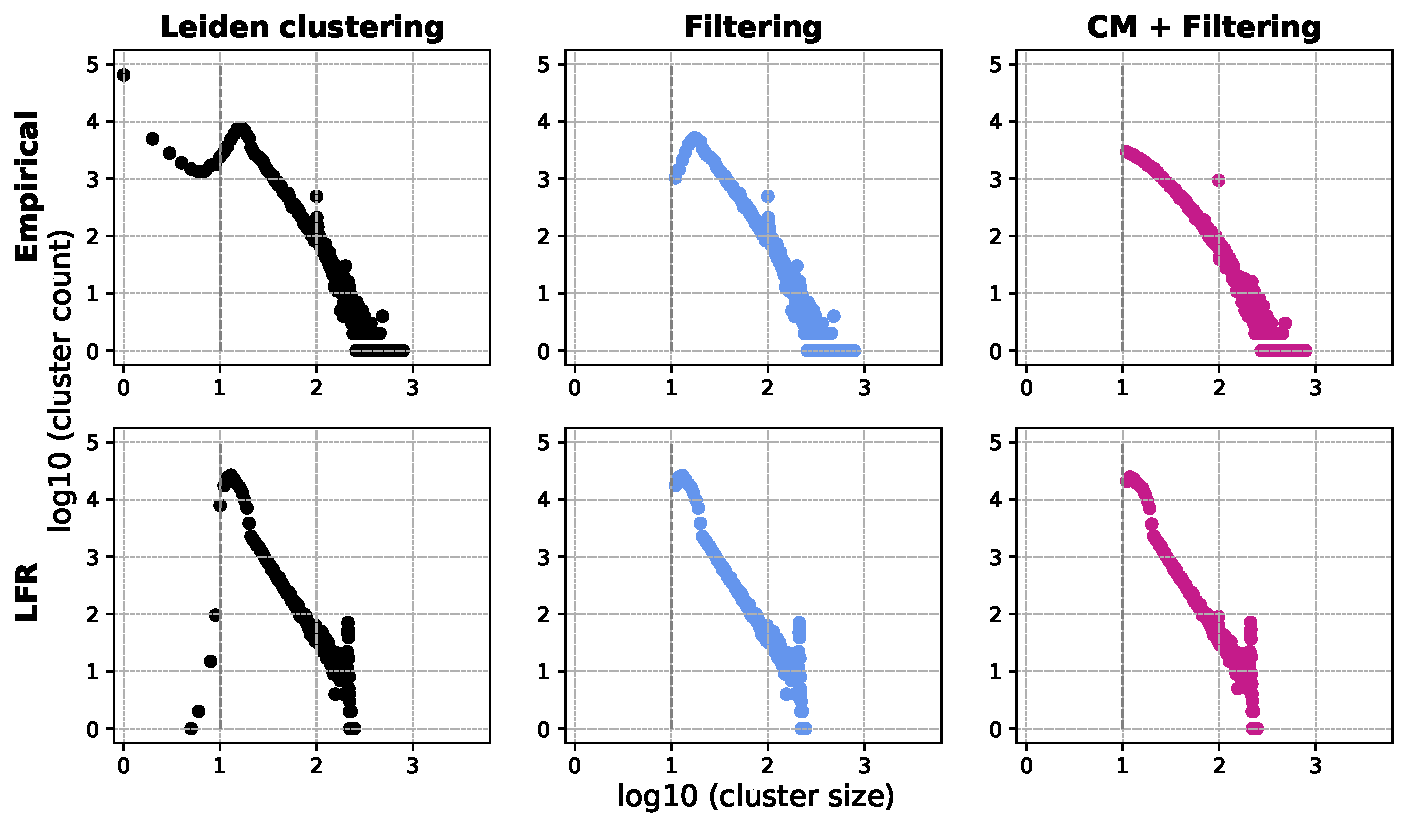
\includegraphics[width=0.62\textwidth]{figs/cit_patents_cm_steps_lfr01.pdf}
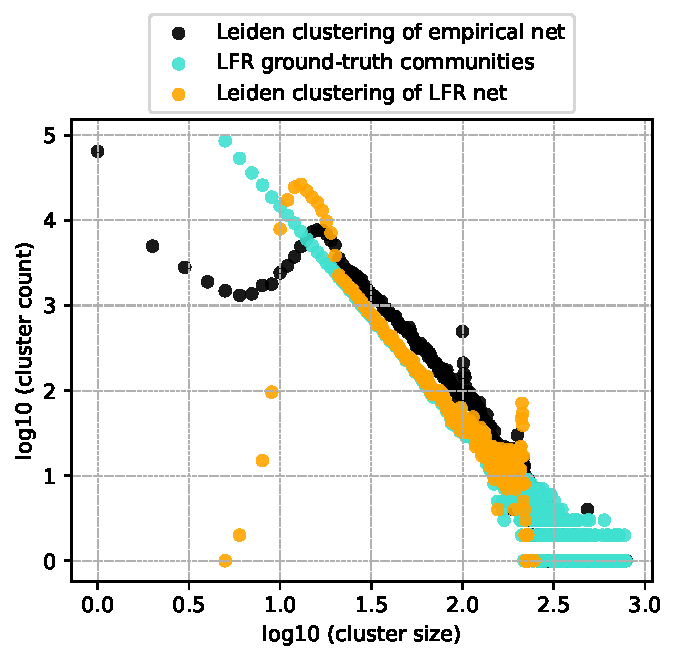
\includegraphics[width=0.37\textwidth]{figs/cit_patents_01_cm_size.pdf}
\caption[CM pipeline on the empirical Citation Patents Network and its model LFR graph for r=0.01]{\textbf{CM pipeline on the empirical Citation Patents network and its model LFR graph for $r=0.01$.} Both networks have 3,774,768 nodes, with an average degree of 8.75 for the empirical network and 8.29 for the LFR graph and both have mixing parameters of 0.382. The left panel shows the community size distribution in each step of running CM and the right panel shows a comparison between the community size distribution of the original Leiden clustering, the LFR ground-truth communities, and the Leiden clustering of the LFR network.}
\label{fig:patents-cm-lfr-01}
\end{figure}

\begin{figure}[h!]
\centering
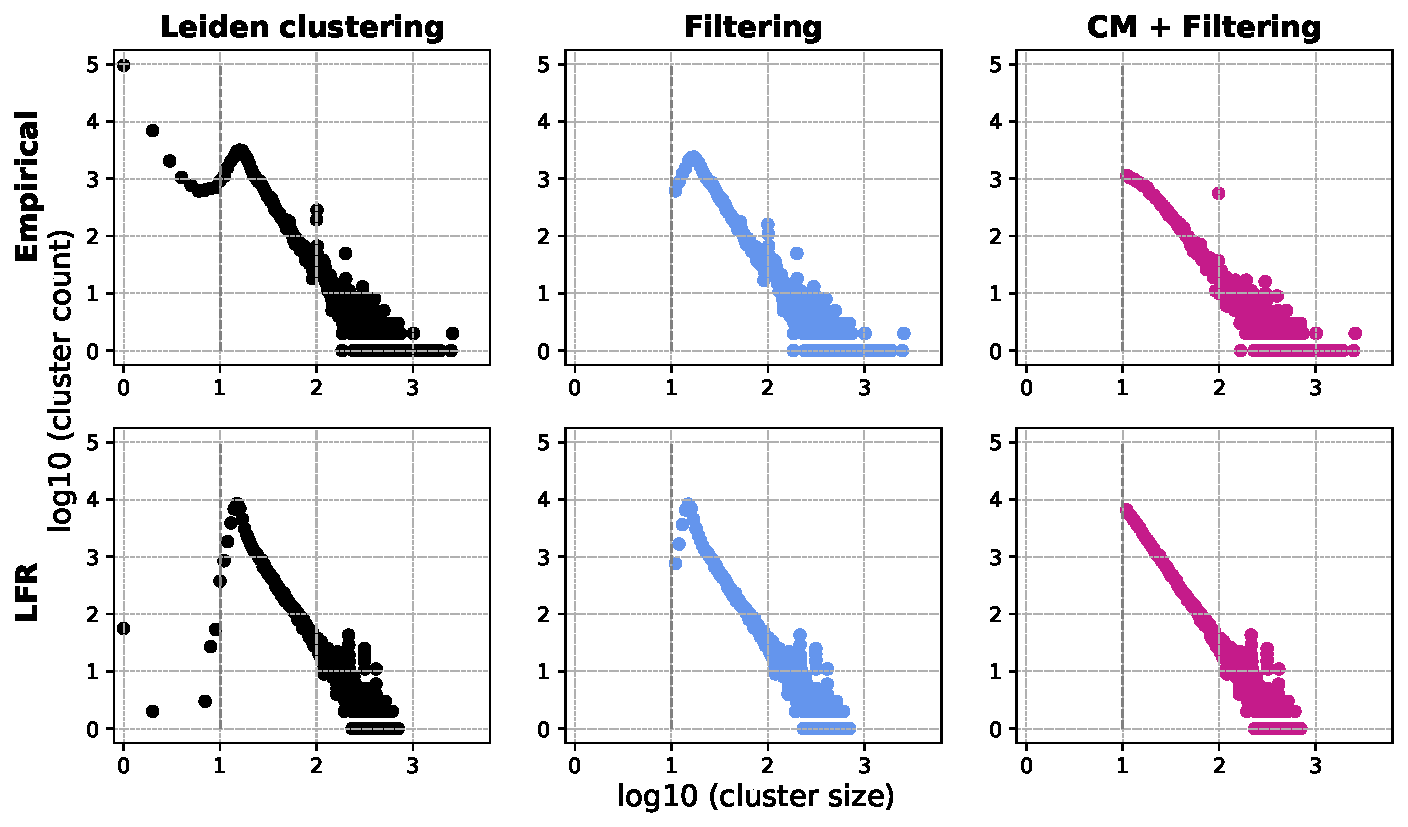
\includegraphics[width=0.62\textwidth]{figs/wiki_topcats_cm_steps_lfr01.pdf}
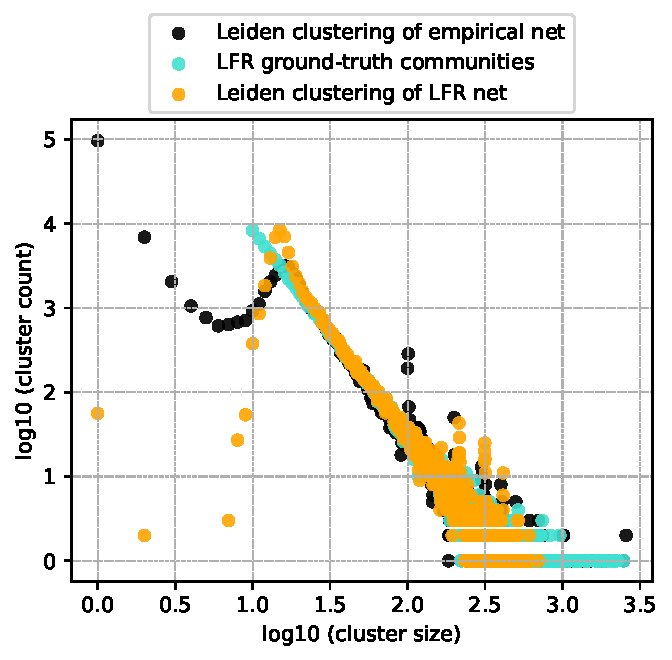
\includegraphics[width=0.37\textwidth]{figs/wiki_topcats_01_cm_size.pdf}
\caption[CM pipeline on the  empirical Wiki-Topcats  network and its model LFR graph for r=0.01]{\textbf{CM pipeline on the empirical Wiki-Topcats network and its model LFR graph for $r=0.01$.} The left panel shows the community size distribution in each step of running CM and the right panel shows a comparison between the community size distribution of the original Leiden clustering, the LFR ground-truth communities, and the Leiden clustering of the LFR network.}
\label{fig:wikitopcats-cm-lfr-01}
\end{figure}

\begin{figure}[h!]
\centering
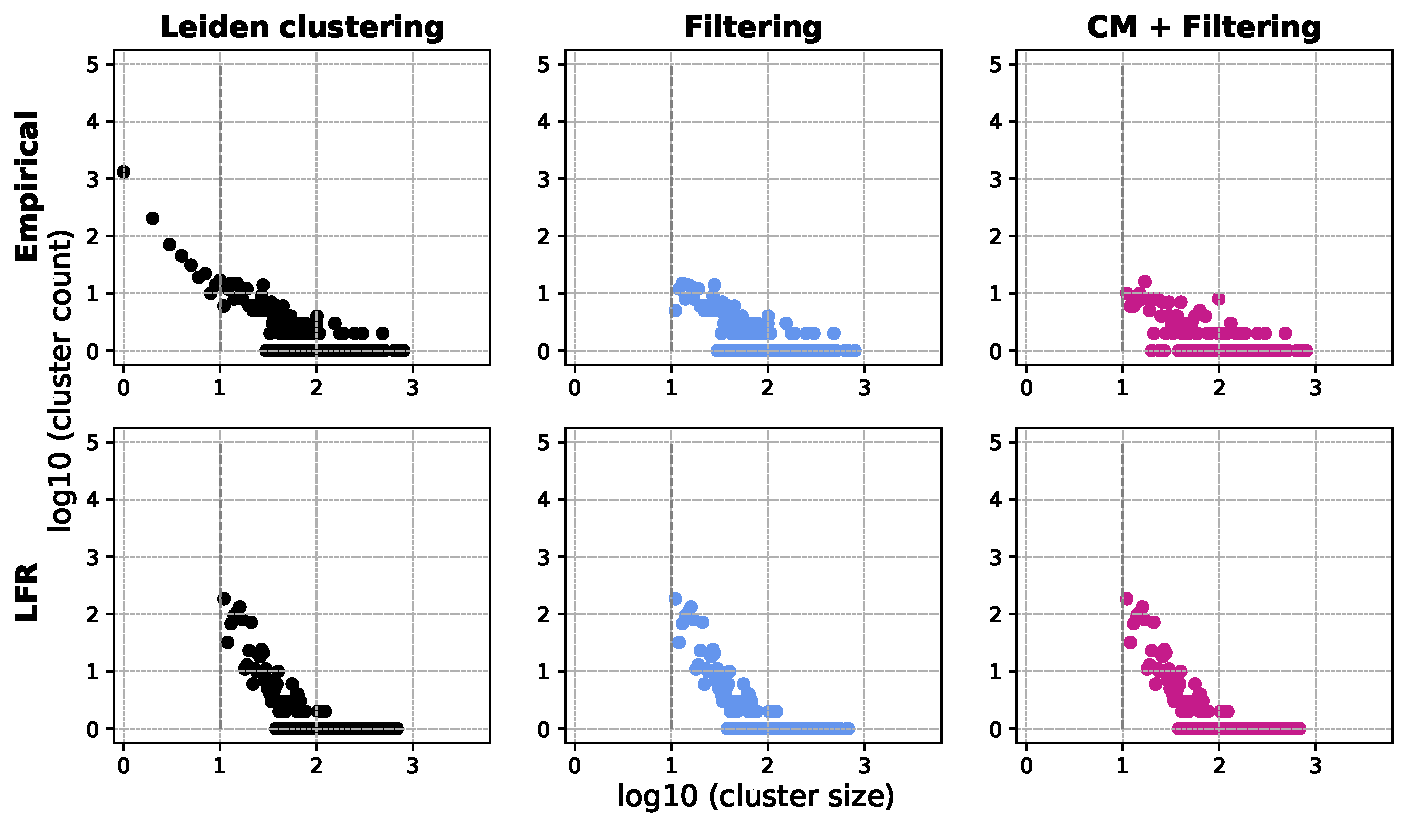
\includegraphics[width=0.62\textwidth]{figs/cit_hepph_cm_steps_lfr01.pdf}
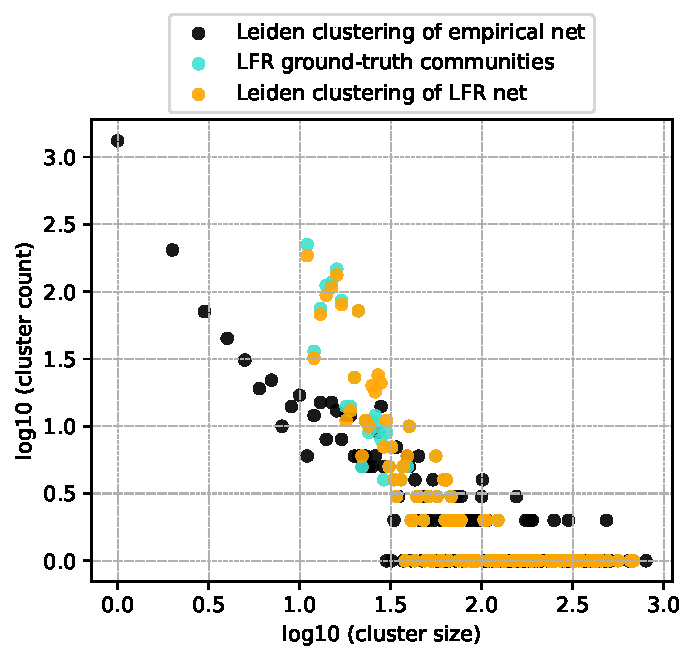
\includegraphics[width=0.37\textwidth]{figs/cit_hepph_01_cm_size.pdf}
\caption[CM pipeline on the empirical High Energy Physics Citation network and its model LFR graph for r=0.01]{\textbf{CM pipeline on the empirical High Energy Physics Citation Network and its model LFR graph for $r=0.01$.} The left panel shows the community size distribution in each step of running CM and the right panel shows a comparison between the community size distribution of the original Leiden clustering, the LFR ground-truth communities, and the Leiden clustering of the LFR network.}
\label{fig:hepph-cm-lfr-01}
\end{figure}

\section{Conclusions}
This study considered the question of how well-connected clusters are when produced by either Leiden or IKC.
When defining well-connected to require  that the smallest edge cut for a cluster with $n$ vertices  have more than $\log_{10}(n)$ edges, we observed that Leiden clusterings
often had many poorly-connected clusters. More specifically, unless the resolution value was large (i.e., $r \geq 0.1$), in the six empirical networks we
considered (two large citation networks and four SNAP networks), at least half the clusters were poorly connected.
We also saw that node coverage dropped as a result of CM-processing.
Although the degree of impact depended on the resolution parameter, this was a consistent pattern across all empirical networks
Moreover, unless the resolution parameter was very large (at least $0.1$ in our experiments), the reduction in node coverage was large.
\textcolor{blue}{This text depends on wishful thinking at this point, because I don't have information on the SNAP networks...so we need these values for the SNAP networks.}

We saw different patterns on the six LFR networks that we simulated based on properties from the corresponding empirical networks.
Although the LFR networks had some small clusters, they had fewer small clusters than those produced on the empirical networks.
The shape of the distributions were also different on the LFR networks than on the empirical networks There were fewer clusters that were considered poorly connected
(according to Equation \ref{eqn:our-bound}), with the result that CPM-processing had a smaller impact on LFR networks than on empirical networks.
In particular, node coverage dropped only slightly, and this drop was primarily due to the filtering out the small clusters.

The findings that LFR networks produce different patterns than empirical networks is perhaps not surprising, but here we posit a few potential explanations.
First, the LFR methodology assumes that every vertex is in a valid community; it also assumes that the degree distribution and cluster size distributions follow some
particular form \textcolor{blue}{Yasamin, to write?}.
These assumptions may not hold on real-world networks.
Future work is needed to best understand why clustering on LFR networks results in such different patterns than on real-world networks.

\section*{Competing Interests} \vspace{3mm} The authors have no competing interests.

\section*{Funding Information} Research in this manuscript was supported by a partnership between the Insper Institute, Brazil and the Department of Computer Science at the University of Illinois Urbana-Champaign. Roughly
50\% of the work was performed in the Oracle Cloud Infrastructure, courtesy of an Oracle Research Award to Tandy Warnow.

\section*{Data Availability}

\section*{Acknowledgments} We thank Christine Ballard, Bryan Barker, and Nathan Bryans from Oracle for their help in setting up and managing a computational environment in the Oracle Cloud Infrastructure.

\bibliographystyle{apalike}
\bibliography{cmv1}
\end{document}


\begin{itemize}
\item For  the CEN and  for the Open Citations networks, produce one LFR network  that has a mixing parameter and other
parameters set so as to produce something that resembles the given Leiden clustering of the given real-world network. (However, keep the LFR network
on the moderate size, so at most 3,000,000 vertices.)

\item
For each LFR network:
\begin{itemize}
\item Report empirical statistics of the network
\item Report empirical statistics of the true clustering
\item Capture accuracy relative to `ground' truth
\item
Recluster using Leiden (same resolution value) and then run the CM pipeline.
Record all the usual statistics
\item Run CM on the true clustering.
Report all the usual statistics
\end{itemize}
\end{itemize}


\noindent
The usual statistics are things like:
\begin{itemize}
\item Statistics before running the CM pipeline, including distribution of cluster sizes, node and edge coverage. \textcolor{red}{node coverage should be defined somewhere. if it has two definitions (nodes in non-singleton clusters, nodes in clusters with size more than 10), mention both. }

\item Statistics at each stage of the CM pipeline (percentage of clusters that are deleted due to being trees,
then deleted due to being too small, then the percentage of remaining clusters  that have small edge cuts).
But at the end of the pipeline we also remove small clusters.
Also show total node and edge coverage at the end of each stage of the CM pipeline.
\item
In essence we want to know which clusters in the input survive the entire process, which ones are modified.
We'll want their sizes as well, so we can say things like ``20\% of the input clusters above size 100 have small edge cuts" and
``10\% of the input clusters above size 50 are trees".
\end{itemize}


% latex table generated in R 4.1.3 by xtable 1.8-4 package
% Sun Jan 22 19:56:56 2023
\begin{table}[ht]
\centering
\resizebox{.5\textwidth}{!}{
\begin{tabular}{rrrrrll}
  \hline
 & clus\_count & min & med & max & type & gp \\
  \hline
1 & 20648920 &   2 &   2 &  10 & size 2-10 & leiden.5 \\
  2 & 297038 &  11 &  13 & 183 & size $>$10 & leiden.5 \\
  3 & 297038 &  11 &  13 & 183 & non\_tree & leiden.5 \\
  4 & 10349 &  11 &  13 &  85 & pre-cm & leiden.5 \\
  5 & 10349 &  11 &  13 &  85 & post-cm & leiden.5 \\
  \hline
  6 & 7324830 &   2 &   5 &  10 & size 2-10 & leiden.1 \\
  7 & 1313856 &  11 &  17 & 882 & size $>$10 & leiden.1 \\
  8 & 1299838 &  11 &  17 & 882 & non\_tree & leiden.1 \\
  9 & 14016 &  11 &  11 &  11 & star & leiden.1 \\
  10 &   2 &  11 &  11 &  11 & tree & leiden.1 \\
  11 & 45252 &  11 &  15 & 306 & pre-cm & leiden.1 \\
  12 & 39954 &  11 &  16 & 306 & post-cm & leiden.1 \\
  \hline
  13 & 772769 &   2 &   2 &  10 &  size 2-10 & leiden.01 \\
  14 & 1361168 &  11 &  19 & 3530 & size $>$10 & leiden.01 \\
  15 & 1034558 &  11 &  24 & 3530 & non\_tree & leiden.01 \\
  16 & 8669 &  11 &  18 & 101 & star & leiden.01 \\
  17 & 317941 &  11 &  15 &  58 & tree & leiden.01 \\
  18 & 36171 &  11 &  21 & 1561 & pre-cm & leiden.01 \\
  19 & 29793 &  11 &  16 & 1561 & post-cm & leiden.01 \\
  \hline
  20 & 606966 &   2 &   2 &  10 & size 2-10 & leiden.001 \\
  21 & 232288 &  11 &  64 & 23470 & size $>$10  & leiden.001 \\
  22 & 208543 &  11 &  73 & 23470 & non\_tree & leiden.001 \\
  23 & 1476 &  11 &  15 & 1001 & star & leiden.001 \\
  24 & 22269 &  11 &  43 & 500 & tree & leiden.001 \\
  25 & 7299 &  11 &  63 & 12707 & pre-cm & leiden.001 \\
  26 & 11766 &  11 &  43 & 12707 & post-cm & leiden.001 \\
  \hline
  27 & 522696 &   2 &   2 &  10 & size 2-10 & leiden.0001 \\
  28 & 39069 &  11 & 177 & 176557 & size $>$10 & leiden.0001 \\
  29 & 34031 &  11 & 206 & 176557 & non\_tree & leiden.0001 \\
  30 & 3525 &  11 &  14 & 267 & tree & leiden.0001 \\
  31 & 1513 &  11 &  14 & 251 & star & leiden.0001 \\
  32 & 1192 &  11 & 172 & 53195 & pre-cm & leiden.0001 \\
  33 & 1971 &  11 & 118 & 51053 & post-cm & leiden.0001 \\
   \hline
\end{tabular}}
\caption{test- data being revised to use larger samples}
\end{table}


\paragraph{SNAP benchmarks}
In addition, five more real world networks from the Stanford Network Analysis Project (SNAP) collection \citep{leskovec2016snap} were downloaded in Dec 2022:
\begin{itemize}
\item  \emph{cit\_patents} (3,774,768 nodes, 16,518,947 edges), \
\item \emph{cit\_hepph} (34,546 nodes, 420,877 edges),
\item  \emph{wiki\_topcats} (1,791,489 nodes, 25,444,207 edges)
\item  \emph{orkut} (3,072,441 nodes, 117,185,083 edges).
\item \emph{wiki\_talk} (2,394,385 nodes, 4,659,565 edges)
\end{itemize}

\begin{table}[ht]
\centering
\begin{tabular}{rlrrrrrrr}
  \hline
 & clustering & n=1 & n$>$1 & n$\geq 11$ & min & med & max & node\_cov \\
  \hline
1 & leiden 0.5 & 12,701,653 & 433,557 & 8,503 & 11 & 14 & 68 & 0.97 \\
  2 & leiden 0.1 & 8,341,818 & 516,299 & 273,420 & 11 & 11 & 319 & 23.98 \\
  3 & leiden 0.01 & 3,245,556 & 280,518 & 275,641 & 11 & 28 & 3,186 & 76.52 \\
  4 & leiden 0.001 & 2,172,927 & 66,326 & 65,771 & 11 & 98 & 16,481 & 84.45 \\
   \hline
\end{tabular}
\caption{Statistics on Leiden clusters of the Curated Exosome Network (CEN).
We show number of non-singleton clusters ($n >1$) and number of clusters of size at least 11, as well as minimum, median, and
maximum cluster size when restricted to clusters of size at least $11$. The node coverage refers to percentage of nodes in the CEN found in clusters of size at least 11.
Node coverage and cluster size increase as resolution values is decreased. The first column (clustering) shows the resolution value passed as a parameter to Leiden. The next three columns show cluster counts for singleton clusters, non-singleton clusters, and clusters of size at least 11. Minimum, median, and max cluster sizes are shown for clusters of size at least 11. The last column indicates node coverage expressed as a percentage; the count of nodes in clusters of size at least 11, relative to the total number of nodes in the network.}
\label{tab:CEN-table1}
\end{table}



\paragraph{Searching for Trees in the CEN}
\textcolor{blue}{George, if we are going to do this for the CEN, shouldn't we be doing this for Open Citations? }
We also explored whether trees, which are extreme examples of poorly connected clusters, were being generated. Accordingly, we searched for trees in clusterings generated by  Leiden.
We filtered out clusters of size at most 10 before evaluating clusters for the presence of trees. Strikingly, we observed trees in Leiden clusterings from resolution values of 0.1, 0.01, and 0.001 but not at 0.5. At resolution value of 0.1, 273,420 clusters were generated of which 254,734 (93.2\%) were trees of size 11. At a resolution value of 0.001, 65,771 clusters were generated were found, of which 22,750 (34.6\%) were
trees (Figure \ref{fig:trees-in-networks} and Table \ref{tab:CEN-table2}.)
 Interestingly, as resolution values were decreased further, the number of trees decreased but the average tree size increased (Figure \ref{somefig}, Table \ref{tab:CEN-table3}).

\begin{figure}[h]
\centering
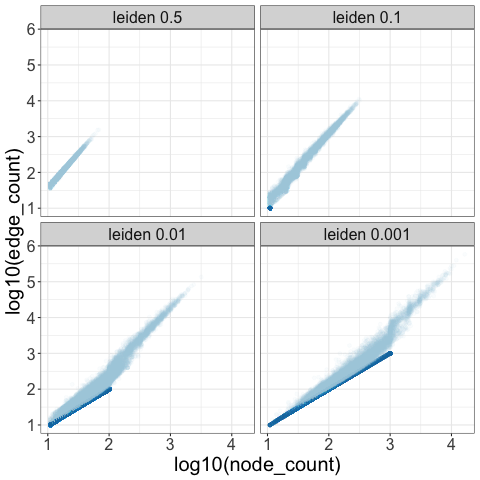
\includegraphics[width=0.4\linewidth]{figs/cen_quad_fig1.png}
\caption{Edge-density of Leiden clusters of the CEN at four resolution values (0.5, 0.1, 0.01, 0.001).
%with CPM as quality function.
The figure shows the count of nodes in each cluster plotted against the number of edges in each cluster, restricted to clusters of size at least 11;  dark blue indicates tree clusters, light blue indicates other clusters.
%As resolution value decreases, node coverage (the fraction of nodes that are found in clusters of size at least 11) increases. The number of such clusters does not, however, monotonically increase (Table \ref{tab:CEN-table1}).
No trees are found for the largest resolution value, but as the resolution value decreases, tree clusters are detected at increasing size.
%with maximum tree size inversely related to resolution value. However, the number of trees decreases as the resolution factor is decreased, with the exception of clustering at 0.5 for which no trees are detected
See Table   \ref{tab:CEN-Leiden-11-CM} for additional statistics.}
\label{fig:Leiden-CEN-trees}
%The Curated Exosome Network (CEN) consists of 13,989,436 nodes and 92,051,051 edges. The average degree of its nodes is 13.16.
\end{figure}

To follow up on the presence of sparse clusters in the form of trees, Leiden clusters were filtered to exclude clusters of size at most 10, after which the number of clusters that were \emph{trees} (ti.e., clusters that have no cycles, equivalently the case where he number of nodes in a cluster is exactly  one more than the number of intra-cluster edges) were counted. Trees were then filtered, after which the remaining clusters were processed with connectivity modifier (CM) using Equation \ref{eqn:our-bound} as the threshold, then filtered again to remove small clusters (Table \ref{tab:CEN-Leiden-11-CM}).

% latex table generated in R 4.1.3 by xtable 1.8-4 package
% Sun Jan 29 23:08:57 2023
% generated by running table2.R on odesa in
% /data1/snap_leiden_venv/cen

\clearpage

\begin{table}[H]
\centering
\begin{tabular}{lrllrrr}
  \hline
 Clustering & Resolution & type & min & med & max \\
  \hline
leiden & 0.5 & non\_tree &  11 & 14 &  68 \\
leiden & 0.5 & tree &  NA & NA &  NA \\
leiden & 0.1 & tree &  11 & 11 &  11 \\
leiden  & 0.1 & non\_tree &  11 & 20 & 319 \\
leiden  & 0.01 & tree &  11 & 27 & 101 \\
leiden & 0.01 & non\_tree &  11 & 34 & 3186 \\
leiden & 0.001 & tree &  11 & 65 & 1001 \\
leiden & 0.001 & non\_tree &  12 & 112 & 16481 \\

   \hline
\end{tabular}
\caption{Leiden clusters on the CEN, based on whether the cluster is a tree. We show empirical statistics (minimum, median, and maximum) of Leiden clusters generated using the Constant Potts Model (CPM) as quality function and with different resolution values. Clusters of of size at most 10 have been removed. Do we need this table?}
\end{table}

\clearpage
